\documentclass[twoside]{book}

% Packages required by doxygen
\usepackage{calc}
\usepackage{doxygen}
\usepackage{graphicx}
\usepackage[utf8]{inputenc}
\usepackage{makeidx}
\usepackage{multicol}
\usepackage{multirow}
\usepackage{textcomp}
\usepackage[table]{xcolor}

% Font selection
\usepackage[T1]{fontenc}
\usepackage{mathptmx}
\usepackage[scaled=.90]{helvet}
\usepackage{courier}
\usepackage{amssymb}
\usepackage{sectsty}
\renewcommand{\familydefault}{\sfdefault}
\allsectionsfont{%
  \fontseries{bc}\selectfont%
  \color{darkgray}%
}
\renewcommand{\DoxyLabelFont}{%
  \fontseries{bc}\selectfont%
  \color{darkgray}%
}

% Page & text layout
\usepackage{geometry}
\geometry{%
  a4paper,%
  top=2.5cm,%
  bottom=2.5cm,%
  left=2.5cm,%
  right=2.5cm%
}
\tolerance=750
\hfuzz=15pt
\hbadness=750
\setlength{\emergencystretch}{15pt}
\setlength{\parindent}{0cm}
\setlength{\parskip}{0.2cm}
\makeatletter
\renewcommand{\paragraph}{%
  \@startsection{paragraph}{4}{0ex}{-1.0ex}{1.0ex}{%
    \normalfont\normalsize\bfseries\SS@parafont%
  }%
}
\renewcommand{\subparagraph}{%
  \@startsection{subparagraph}{5}{0ex}{-1.0ex}{1.0ex}{%
    \normalfont\normalsize\bfseries\SS@subparafont%
  }%
}
\makeatother

% Headers & footers
\usepackage{fancyhdr}
\pagestyle{fancyplain}
\fancyhead[LE]{\fancyplain{}{\bfseries\thepage}}
\fancyhead[CE]{\fancyplain{}{}}
\fancyhead[RE]{\fancyplain{}{\bfseries\leftmark}}
\fancyhead[LO]{\fancyplain{}{\bfseries\rightmark}}
\fancyhead[CO]{\fancyplain{}{}}
\fancyhead[RO]{\fancyplain{}{\bfseries\thepage}}
\fancyfoot[LE]{\fancyplain{}{}}
\fancyfoot[CE]{\fancyplain{}{}}
\fancyfoot[RE]{\fancyplain{}{\bfseries\scriptsize Generated on Mon May 20 2013 12:01:50 for Omega Wars by Doxygen }}
\fancyfoot[LO]{\fancyplain{}{\bfseries\scriptsize Generated on Mon May 20 2013 12:01:50 for Omega Wars by Doxygen }}
\fancyfoot[CO]{\fancyplain{}{}}
\fancyfoot[RO]{\fancyplain{}{}}
\renewcommand{\footrulewidth}{0.4pt}
\renewcommand{\chaptermark}[1]{%
  \markboth{#1}{}%
}
\renewcommand{\sectionmark}[1]{%
  \markright{\thesection\ #1}%
}

% Indices & bibliography
\usepackage{natbib}
\usepackage[titles]{tocloft}
\setcounter{tocdepth}{3}
\setcounter{secnumdepth}{5}
\makeindex

% Hyperlinks (required, but should be loaded last)
\usepackage{ifpdf}
\ifpdf
  \usepackage[pdftex,pagebackref=true]{hyperref}
\else
  \usepackage[ps2pdf,pagebackref=true]{hyperref}
\fi
\hypersetup{%
  colorlinks=true,%
  linkcolor=blue,%
  citecolor=blue,%
  unicode%
}

% Custom commands
\newcommand{\clearemptydoublepage}{%
  \newpage{\pagestyle{empty}\cleardoublepage}%
}


%===== C O N T E N T S =====

\begin{document}

% Titlepage & ToC
\hypersetup{pageanchor=false}
\pagenumbering{roman}
\begin{titlepage}
\vspace*{7cm}
\begin{center}%
{\Large Omega Wars }\\
\vspace*{1cm}
{\large Generated by Doxygen 1.8.4}\\
\vspace*{0.5cm}
{\small Mon May 20 2013 12:01:50}\\
\end{center}
\end{titlepage}
\clearemptydoublepage
\tableofcontents
\clearemptydoublepage
\pagenumbering{arabic}
\hypersetup{pageanchor=true}

%--- Begin generated contents ---
\chapter{Hierarchical Index}
\section{Class Hierarchy}
This inheritance list is sorted roughly, but not completely, alphabetically\-:\begin{DoxyCompactList}
\item \contentsline{section}{Bullet}{\pageref{class_bullet}}{}
\item \contentsline{section}{Enemy}{\pageref{class_enemy}}{}
\item \contentsline{section}{intromessage}{\pageref{classintromessage}}{}
\item \contentsline{section}{location}{\pageref{structlocation}}{}
\item \contentsline{section}{Player}{\pageref{class_player}}{}
\item \contentsline{section}{Score}{\pageref{struct_score}}{}
\item \contentsline{section}{Scoring}{\pageref{class_scoring}}{}
\item \contentsline{section}{Sound\-F\-X\-Manager}{\pageref{class_sound_f_x_manager}}{}
\item \contentsline{section}{World}{\pageref{class_world}}{}
\begin{DoxyCompactList}
\item \contentsline{section}{Intro\-Menu}{\pageref{class_intro_menu}}{}
\end{DoxyCompactList}
\end{DoxyCompactList}

\chapter{Class Index}
\section{Class List}
Here are the classes, structs, unions and interfaces with brief descriptions\-:\begin{DoxyCompactList}
\item\contentsline{section}{\hyperlink{class_bullet}{Bullet} }{\pageref{class_bullet}}{}
\item\contentsline{section}{\hyperlink{class_enemy}{Enemy} }{\pageref{class_enemy}}{}
\item\contentsline{section}{\hyperlink{class_intro_menu}{Intro\-Menu} }{\pageref{class_intro_menu}}{}
\item\contentsline{section}{\hyperlink{classintromessage}{intromessage} }{\pageref{classintromessage}}{}
\item\contentsline{section}{\hyperlink{structlocation}{location} }{\pageref{structlocation}}{}
\item\contentsline{section}{\hyperlink{class_player}{Player} }{\pageref{class_player}}{}
\item\contentsline{section}{\hyperlink{struct_score}{Score} }{\pageref{struct_score}}{}
\item\contentsline{section}{\hyperlink{class_scoring}{Scoring} }{\pageref{class_scoring}}{}
\item\contentsline{section}{\hyperlink{class_sound_f_x_manager}{Sound\-F\-X\-Manager} }{\pageref{class_sound_f_x_manager}}{}
\item\contentsline{section}{\hyperlink{class_world}{World} }{\pageref{class_world}}{}
\end{DoxyCompactList}

\chapter{File Index}
\section{File List}
Here is a list of all files with brief descriptions\-:\begin{DoxyCompactList}
\item\contentsline{section}{C\-:/\-Users/\-Clarke/\-Documents/\-Codeblocks/\-O\-Omap\-Game/\hyperlink{main_8cpp}{main.\-cpp} }{\pageref{main_8cpp}}{}
\item\contentsline{section}{C\-:/\-Users/\-Clarke/\-Documents/\-Codeblocks/\-O\-Omap\-Game/\hyperlink{resources_8cpp}{resources.\-cpp} }{\pageref{resources_8cpp}}{}
\item\contentsline{section}{C\-:/\-Users/\-Clarke/\-Documents/\-Codeblocks/\-O\-Omap\-Game/\hyperlink{resources_8h}{resources.\-h} }{\pageref{resources_8h}}{}
\item\contentsline{section}{C\-:/\-Users/\-Clarke/\-Documents/\-Codeblocks/\-O\-Omap\-Game/\hyperlink{world__bullet_8cpp}{world\-\_\-bullet.\-cpp} }{\pageref{world__bullet_8cpp}}{}
\item\contentsline{section}{C\-:/\-Users/\-Clarke/\-Documents/\-Codeblocks/\-O\-Omap\-Game/\hyperlink{world__enemy_8cpp}{world\-\_\-enemy.\-cpp} }{\pageref{world__enemy_8cpp}}{}
\item\contentsline{section}{C\-:/\-Users/\-Clarke/\-Documents/\-Codeblocks/\-O\-Omap\-Game/include/\hyperlink{bullet_8h}{bullet.\-h} }{\pageref{bullet_8h}}{}
\item\contentsline{section}{C\-:/\-Users/\-Clarke/\-Documents/\-Codeblocks/\-O\-Omap\-Game/include/\hyperlink{enemy_8h}{enemy.\-h} }{\pageref{enemy_8h}}{}
\item\contentsline{section}{C\-:/\-Users/\-Clarke/\-Documents/\-Codeblocks/\-O\-Omap\-Game/include/\hyperlink{intromenu_8h}{intromenu.\-h} }{\pageref{intromenu_8h}}{}
\item\contentsline{section}{C\-:/\-Users/\-Clarke/\-Documents/\-Codeblocks/\-O\-Omap\-Game/include/\hyperlink{intromessage_8h}{intromessage.\-h} }{\pageref{intromessage_8h}}{}
\item\contentsline{section}{C\-:/\-Users/\-Clarke/\-Documents/\-Codeblocks/\-O\-Omap\-Game/include/\hyperlink{player_8h}{player.\-h} }{\pageref{player_8h}}{}
\item\contentsline{section}{C\-:/\-Users/\-Clarke/\-Documents/\-Codeblocks/\-O\-Omap\-Game/include/\hyperlink{scoring_8h}{scoring.\-h} }{\pageref{scoring_8h}}{}
\item\contentsline{section}{C\-:/\-Users/\-Clarke/\-Documents/\-Codeblocks/\-O\-Omap\-Game/include/\hyperlink{soundmanager_8h}{soundmanager.\-h} }{\pageref{soundmanager_8h}}{}
\item\contentsline{section}{C\-:/\-Users/\-Clarke/\-Documents/\-Codeblocks/\-O\-Omap\-Game/include/\hyperlink{world_8h}{world.\-h} }{\pageref{world_8h}}{}
\item\contentsline{section}{C\-:/\-Users/\-Clarke/\-Documents/\-Codeblocks/\-O\-Omap\-Game/src/\hyperlink{bullet_8cpp}{bullet.\-cpp} }{\pageref{bullet_8cpp}}{}
\item\contentsline{section}{C\-:/\-Users/\-Clarke/\-Documents/\-Codeblocks/\-O\-Omap\-Game/src/\hyperlink{enemy_8cpp}{enemy.\-cpp} }{\pageref{enemy_8cpp}}{}
\item\contentsline{section}{C\-:/\-Users/\-Clarke/\-Documents/\-Codeblocks/\-O\-Omap\-Game/src/\hyperlink{intromenu_8cpp}{intromenu.\-cpp} }{\pageref{intromenu_8cpp}}{}
\item\contentsline{section}{C\-:/\-Users/\-Clarke/\-Documents/\-Codeblocks/\-O\-Omap\-Game/src/\hyperlink{intromessage_8cpp}{intromessage.\-cpp} }{\pageref{intromessage_8cpp}}{}
\item\contentsline{section}{C\-:/\-Users/\-Clarke/\-Documents/\-Codeblocks/\-O\-Omap\-Game/src/\hyperlink{player_8cpp}{player.\-cpp} }{\pageref{player_8cpp}}{}
\item\contentsline{section}{C\-:/\-Users/\-Clarke/\-Documents/\-Codeblocks/\-O\-Omap\-Game/src/\hyperlink{scoring_8cpp}{scoring.\-cpp} }{\pageref{scoring_8cpp}}{}
\item\contentsline{section}{C\-:/\-Users/\-Clarke/\-Documents/\-Codeblocks/\-O\-Omap\-Game/src/\hyperlink{soundmanager_8cpp}{soundmanager.\-cpp} }{\pageref{soundmanager_8cpp}}{}
\item\contentsline{section}{C\-:/\-Users/\-Clarke/\-Documents/\-Codeblocks/\-O\-Omap\-Game/src/\hyperlink{world_8cpp}{world.\-cpp} }{\pageref{world_8cpp}}{}
\end{DoxyCompactList}

\chapter{Class Documentation}
\hypertarget{class_bullet}{\section{Bullet Class Reference}
\label{class_bullet}\index{Bullet@{Bullet}}
}


{\ttfamily \#include $<$bullet.\-h$>$}

\subsection*{Public Member Functions}
\begin{DoxyCompactItemize}
\item 
\hyperlink{class_bullet_acd7befc0bc18907cc1d871d37bbdddeb}{Bullet} ()
\item 
\hyperlink{structlocation}{location} \hyperlink{class_bullet_a7d5f75b11e8506b81c0d09d0f6954631}{get\-Location} ()
\item 
\hyperlink{structlocation}{location} \hyperlink{class_bullet_a6605541b9caf5ce0d0f04f42ccefedd3}{get\-Prev\-Location} ()
\item 
char \hyperlink{class_bullet_ae63d1923f5b35f0b27ef629a384e8405}{get\-Appearance} ()
\item 
void \hyperlink{class_bullet_aecb7dac661d83c26904f09f14fbb05cd}{set\-Location} (\hyperlink{structlocation}{location} new\-Loc)
\end{DoxyCompactItemize}


\subsection{Detailed Description}


Definition at line 6 of file bullet.\-h.



\subsection{Constructor \& Destructor Documentation}
\hypertarget{class_bullet_acd7befc0bc18907cc1d871d37bbdddeb}{\index{Bullet@{Bullet}!Bullet@{Bullet}}
\index{Bullet@{Bullet}!Bullet@{Bullet}}
\subsubsection[{Bullet}]{\setlength{\rightskip}{0pt plus 5cm}Bullet\-::\-Bullet (
\begin{DoxyParamCaption}
{}
\end{DoxyParamCaption}
)}}\label{class_bullet_acd7befc0bc18907cc1d871d37bbdddeb}


Definition at line 3 of file bullet.\-cpp.



\subsection{Member Function Documentation}
\hypertarget{class_bullet_ae63d1923f5b35f0b27ef629a384e8405}{\index{Bullet@{Bullet}!get\-Appearance@{get\-Appearance}}
\index{get\-Appearance@{get\-Appearance}!Bullet@{Bullet}}
\subsubsection[{get\-Appearance}]{\setlength{\rightskip}{0pt plus 5cm}char Bullet\-::get\-Appearance (
\begin{DoxyParamCaption}
{}
\end{DoxyParamCaption}
)\hspace{0.3cm}{\ttfamily [inline]}}}\label{class_bullet_ae63d1923f5b35f0b27ef629a384e8405}


Definition at line 18 of file bullet.\-h.

\hypertarget{class_bullet_a7d5f75b11e8506b81c0d09d0f6954631}{\index{Bullet@{Bullet}!get\-Location@{get\-Location}}
\index{get\-Location@{get\-Location}!Bullet@{Bullet}}
\subsubsection[{get\-Location}]{\setlength{\rightskip}{0pt plus 5cm}{\bf location} Bullet\-::get\-Location (
\begin{DoxyParamCaption}
{}
\end{DoxyParamCaption}
)\hspace{0.3cm}{\ttfamily [inline]}}}\label{class_bullet_a7d5f75b11e8506b81c0d09d0f6954631}


Definition at line 15 of file bullet.\-h.

\hypertarget{class_bullet_a6605541b9caf5ce0d0f04f42ccefedd3}{\index{Bullet@{Bullet}!get\-Prev\-Location@{get\-Prev\-Location}}
\index{get\-Prev\-Location@{get\-Prev\-Location}!Bullet@{Bullet}}
\subsubsection[{get\-Prev\-Location}]{\setlength{\rightskip}{0pt plus 5cm}{\bf location} Bullet\-::get\-Prev\-Location (
\begin{DoxyParamCaption}
{}
\end{DoxyParamCaption}
)\hspace{0.3cm}{\ttfamily [inline]}}}\label{class_bullet_a6605541b9caf5ce0d0f04f42ccefedd3}


Definition at line 16 of file bullet.\-h.

\hypertarget{class_bullet_aecb7dac661d83c26904f09f14fbb05cd}{\index{Bullet@{Bullet}!set\-Location@{set\-Location}}
\index{set\-Location@{set\-Location}!Bullet@{Bullet}}
\subsubsection[{set\-Location}]{\setlength{\rightskip}{0pt plus 5cm}void Bullet\-::set\-Location (
\begin{DoxyParamCaption}
\item[{{\bf location}}]{new\-Loc}
\end{DoxyParamCaption}
)\hspace{0.3cm}{\ttfamily [inline]}}}\label{class_bullet_aecb7dac661d83c26904f09f14fbb05cd}


Definition at line 20 of file bullet.\-h.



The documentation for this class was generated from the following files\-:\begin{DoxyCompactItemize}
\item 
C\-:/\-Users/\-Clarke/\-Documents/\-Codeblocks/\-O\-Omap\-Game/include/\hyperlink{bullet_8h}{bullet.\-h}\item 
C\-:/\-Users/\-Clarke/\-Documents/\-Codeblocks/\-O\-Omap\-Game/src/\hyperlink{bullet_8cpp}{bullet.\-cpp}\end{DoxyCompactItemize}

\hypertarget{class_enemy}{\section{Enemy Class Reference}
\label{class_enemy}\index{Enemy@{Enemy}}
}


{\ttfamily \#include $<$enemy.\-h$>$}

\subsection*{Public Member Functions}
\begin{DoxyCompactItemize}
\item 
\hyperlink{class_enemy_a94f30d348b6d2840fd71675472ba38dd}{Enemy} ()
\item 
char \hyperlink{class_enemy_a9f821c02c5451799ea348dcf501a7f4c}{get\-Appearance} ()
\item 
\hyperlink{structlocation}{location} \hyperlink{class_enemy_aa93808890d81f5c4a57781e04a29d834}{get\-Location} ()
\item 
\hyperlink{structlocation}{location} \hyperlink{class_enemy_a3d72fece88a3be2561a7952477b6d793}{get\-Prev\-Location} ()
\item 
void \hyperlink{class_enemy_a30f503ca7f6d7a736a81bd6d053d4e18}{set\-Location} (\hyperlink{structlocation}{location} new\-Loc)
\end{DoxyCompactItemize}


\subsection{Detailed Description}


Definition at line 6 of file enemy.\-h.



\subsection{Constructor \& Destructor Documentation}
\hypertarget{class_enemy_a94f30d348b6d2840fd71675472ba38dd}{\index{Enemy@{Enemy}!Enemy@{Enemy}}
\index{Enemy@{Enemy}!Enemy@{Enemy}}
\subsubsection[{Enemy}]{\setlength{\rightskip}{0pt plus 5cm}Enemy\-::\-Enemy (
\begin{DoxyParamCaption}
{}
\end{DoxyParamCaption}
)}}\label{class_enemy_a94f30d348b6d2840fd71675472ba38dd}


Definition at line 3 of file enemy.\-cpp.



\subsection{Member Function Documentation}
\hypertarget{class_enemy_a9f821c02c5451799ea348dcf501a7f4c}{\index{Enemy@{Enemy}!get\-Appearance@{get\-Appearance}}
\index{get\-Appearance@{get\-Appearance}!Enemy@{Enemy}}
\subsubsection[{get\-Appearance}]{\setlength{\rightskip}{0pt plus 5cm}char Enemy\-::get\-Appearance (
\begin{DoxyParamCaption}
{}
\end{DoxyParamCaption}
)\hspace{0.3cm}{\ttfamily [inline]}}}\label{class_enemy_a9f821c02c5451799ea348dcf501a7f4c}


Definition at line 15 of file enemy.\-h.

\hypertarget{class_enemy_aa93808890d81f5c4a57781e04a29d834}{\index{Enemy@{Enemy}!get\-Location@{get\-Location}}
\index{get\-Location@{get\-Location}!Enemy@{Enemy}}
\subsubsection[{get\-Location}]{\setlength{\rightskip}{0pt plus 5cm}{\bf location} Enemy\-::get\-Location (
\begin{DoxyParamCaption}
{}
\end{DoxyParamCaption}
)\hspace{0.3cm}{\ttfamily [inline]}}}\label{class_enemy_aa93808890d81f5c4a57781e04a29d834}


Definition at line 17 of file enemy.\-h.

\hypertarget{class_enemy_a3d72fece88a3be2561a7952477b6d793}{\index{Enemy@{Enemy}!get\-Prev\-Location@{get\-Prev\-Location}}
\index{get\-Prev\-Location@{get\-Prev\-Location}!Enemy@{Enemy}}
\subsubsection[{get\-Prev\-Location}]{\setlength{\rightskip}{0pt plus 5cm}{\bf location} Enemy\-::get\-Prev\-Location (
\begin{DoxyParamCaption}
{}
\end{DoxyParamCaption}
)\hspace{0.3cm}{\ttfamily [inline]}}}\label{class_enemy_a3d72fece88a3be2561a7952477b6d793}


Definition at line 18 of file enemy.\-h.

\hypertarget{class_enemy_a30f503ca7f6d7a736a81bd6d053d4e18}{\index{Enemy@{Enemy}!set\-Location@{set\-Location}}
\index{set\-Location@{set\-Location}!Enemy@{Enemy}}
\subsubsection[{set\-Location}]{\setlength{\rightskip}{0pt plus 5cm}void Enemy\-::set\-Location (
\begin{DoxyParamCaption}
\item[{{\bf location}}]{new\-Loc}
\end{DoxyParamCaption}
)\hspace{0.3cm}{\ttfamily [inline]}}}\label{class_enemy_a30f503ca7f6d7a736a81bd6d053d4e18}


Definition at line 20 of file enemy.\-h.



The documentation for this class was generated from the following files\-:\begin{DoxyCompactItemize}
\item 
C\-:/\-Users/\-Clarke/\-Documents/\-Codeblocks/\-O\-Omap\-Game/include/\hyperlink{enemy_8h}{enemy.\-h}\item 
C\-:/\-Users/\-Clarke/\-Documents/\-Codeblocks/\-O\-Omap\-Game/src/\hyperlink{enemy_8cpp}{enemy.\-cpp}\end{DoxyCompactItemize}

\hypertarget{class_intro_menu}{\section{Intro\-Menu Class Reference}
\label{class_intro_menu}\index{Intro\-Menu@{Intro\-Menu}}
}


{\ttfamily \#include $<$intromenu.\-h$>$}

Inheritance diagram for Intro\-Menu\-:\begin{figure}[H]
\begin{center}
\leavevmode
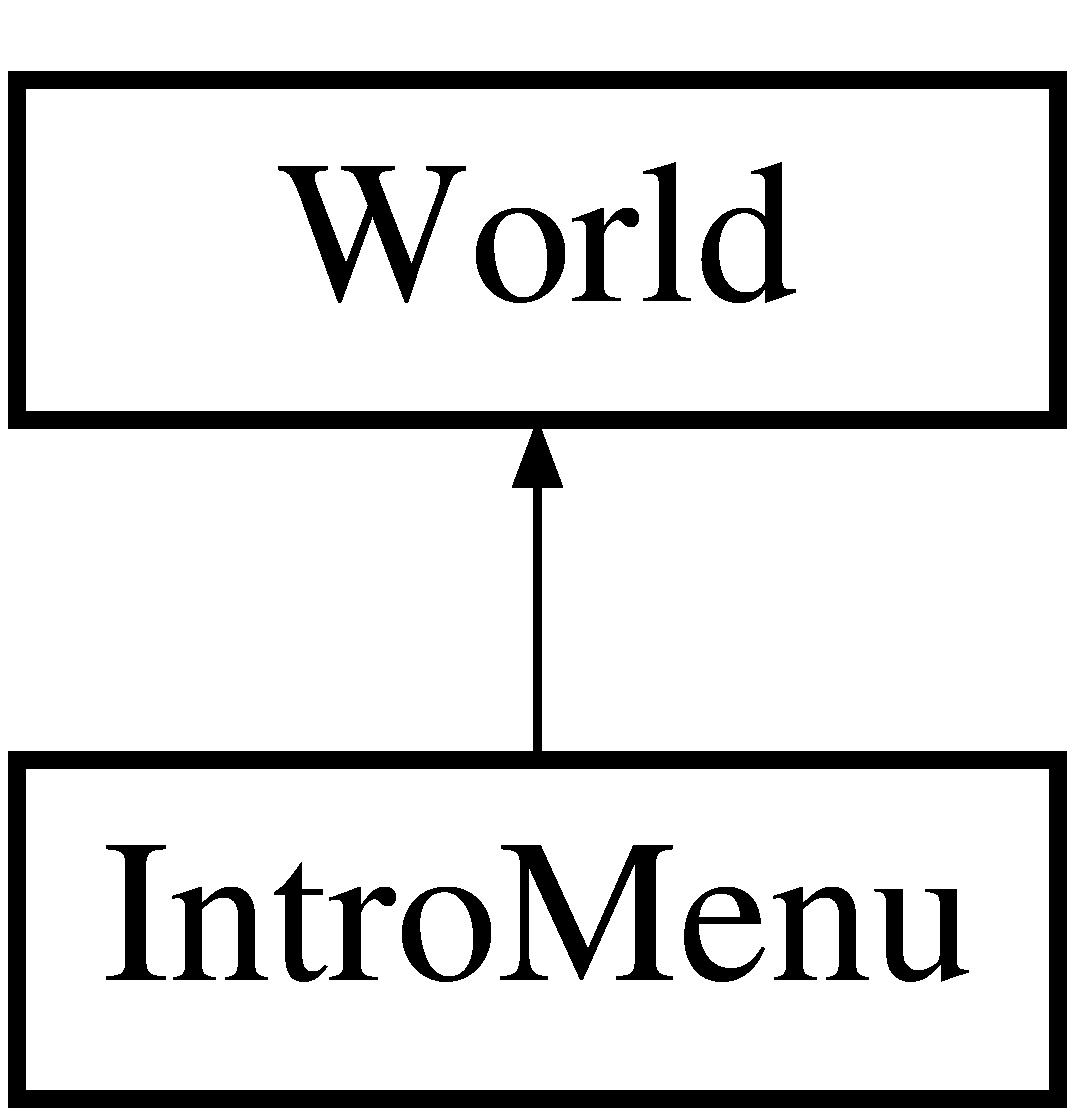
\includegraphics[height=2.000000cm]{class_intro_menu}
\end{center}
\end{figure}
\subsection*{Public Member Functions}
\begin{DoxyCompactItemize}
\item 
\hyperlink{class_intro_menu_ae34d394e4b9c966f44edb891c567a879}{Intro\-Menu} ()
\item 
void \hyperlink{class_intro_menu_aa68a9498b682d93728d31994fed3b032}{display\-Intro\-Screen} ()
\item 
void \hyperlink{class_intro_menu_ad3f2282be033fcac20d1c98bd9bb7cd0}{display\-Message} ()
\item 
int \hyperlink{class_intro_menu_a93b38a1663787bd28b7b64ab04385436}{display\-Options} ()
\end{DoxyCompactItemize}
\subsection*{Additional Inherited Members}


\subsection{Detailed Description}


Definition at line 8 of file intromenu.\-h.



\subsection{Constructor \& Destructor Documentation}
\hypertarget{class_intro_menu_ae34d394e4b9c966f44edb891c567a879}{\index{Intro\-Menu@{Intro\-Menu}!Intro\-Menu@{Intro\-Menu}}
\index{Intro\-Menu@{Intro\-Menu}!IntroMenu@{Intro\-Menu}}
\subsubsection[{Intro\-Menu}]{\setlength{\rightskip}{0pt plus 5cm}Intro\-Menu\-::\-Intro\-Menu (
\begin{DoxyParamCaption}
{}
\end{DoxyParamCaption}
)}}\label{class_intro_menu_ae34d394e4b9c966f44edb891c567a879}


Definition at line 3 of file intromenu.\-cpp.



\subsection{Member Function Documentation}
\hypertarget{class_intro_menu_aa68a9498b682d93728d31994fed3b032}{\index{Intro\-Menu@{Intro\-Menu}!display\-Intro\-Screen@{display\-Intro\-Screen}}
\index{display\-Intro\-Screen@{display\-Intro\-Screen}!IntroMenu@{Intro\-Menu}}
\subsubsection[{display\-Intro\-Screen}]{\setlength{\rightskip}{0pt plus 5cm}void Intro\-Menu\-::display\-Intro\-Screen (
\begin{DoxyParamCaption}
{}
\end{DoxyParamCaption}
)}}\label{class_intro_menu_aa68a9498b682d93728d31994fed3b032}


Definition at line 95 of file intromenu.\-cpp.

\hypertarget{class_intro_menu_ad3f2282be033fcac20d1c98bd9bb7cd0}{\index{Intro\-Menu@{Intro\-Menu}!display\-Message@{display\-Message}}
\index{display\-Message@{display\-Message}!IntroMenu@{Intro\-Menu}}
\subsubsection[{display\-Message}]{\setlength{\rightskip}{0pt plus 5cm}void Intro\-Menu\-::display\-Message (
\begin{DoxyParamCaption}
{}
\end{DoxyParamCaption}
)}}\label{class_intro_menu_ad3f2282be033fcac20d1c98bd9bb7cd0}
Run through dimensions of intro\-Msg

(minus endline char)

Update the map 

Definition at line 109 of file intromenu.\-cpp.

\hypertarget{class_intro_menu_a93b38a1663787bd28b7b64ab04385436}{\index{Intro\-Menu@{Intro\-Menu}!display\-Options@{display\-Options}}
\index{display\-Options@{display\-Options}!IntroMenu@{Intro\-Menu}}
\subsubsection[{display\-Options}]{\setlength{\rightskip}{0pt plus 5cm}int Intro\-Menu\-::display\-Options (
\begin{DoxyParamCaption}
{}
\end{DoxyParamCaption}
)}}\label{class_intro_menu_a93b38a1663787bd28b7b64ab04385436}
Reset the cursor

Run through the dimensions of control menu

Update the map with control menu

Run through the dimensions of options menu

Update the map with options menu

Reset chosen flag

While an option hasnt been chosen

If down was pressed

Clear the current position

Advance teh position

Set the new position

Play selection sound

Play selection sound

If enter was pressed

Play sound

Break out of the loop

Return the selection 

Definition at line 136 of file intromenu.\-cpp.



The documentation for this class was generated from the following files\-:\begin{DoxyCompactItemize}
\item 
C\-:/\-Users/\-Clarke/\-Documents/\-Codeblocks/\-O\-Omap\-Game/include/\hyperlink{intromenu_8h}{intromenu.\-h}\item 
C\-:/\-Users/\-Clarke/\-Documents/\-Codeblocks/\-O\-Omap\-Game/src/\hyperlink{intromenu_8cpp}{intromenu.\-cpp}\end{DoxyCompactItemize}

\hypertarget{classintromessage}{\section{intromessage Class Reference}
\label{classintromessage}\index{intromessage@{intromessage}}
}


{\ttfamily \#include $<$intromessage.\-h$>$}

\subsection*{Public Member Functions}
\begin{DoxyCompactItemize}
\item 
\hyperlink{classintromessage_aabdd5763f78f38cb924a56ccb250ffa9}{intromessage} ()
\item 
int \hyperlink{classintromessage_a311b55407e3d2aa0f906535313867d1b}{get\-Length} ()
\item 
void \hyperlink{classintromessage_af7ca341dc1dcbbc5bf7d8c9c743e0dc3}{show\-Char} (int Char\-Num)
\end{DoxyCompactItemize}


\subsection{Detailed Description}


Definition at line 6 of file intromessage.\-h.



\subsection{Constructor \& Destructor Documentation}
\hypertarget{classintromessage_aabdd5763f78f38cb924a56ccb250ffa9}{\index{intromessage@{intromessage}!intromessage@{intromessage}}
\index{intromessage@{intromessage}!intromessage@{intromessage}}
\subsubsection[{intromessage}]{\setlength{\rightskip}{0pt plus 5cm}intromessage\-::intromessage (
\begin{DoxyParamCaption}
{}
\end{DoxyParamCaption}
)}}\label{classintromessage_aabdd5763f78f38cb924a56ccb250ffa9}


Definition at line 3 of file intromessage.\-cpp.



\subsection{Member Function Documentation}
\hypertarget{classintromessage_a311b55407e3d2aa0f906535313867d1b}{\index{intromessage@{intromessage}!get\-Length@{get\-Length}}
\index{get\-Length@{get\-Length}!intromessage@{intromessage}}
\subsubsection[{get\-Length}]{\setlength{\rightskip}{0pt plus 5cm}int intromessage\-::get\-Length (
\begin{DoxyParamCaption}
{}
\end{DoxyParamCaption}
)\hspace{0.3cm}{\ttfamily [inline]}}}\label{classintromessage_a311b55407e3d2aa0f906535313867d1b}


Definition at line 20 of file intromessage.\-h.

\hypertarget{classintromessage_af7ca341dc1dcbbc5bf7d8c9c743e0dc3}{\index{intromessage@{intromessage}!show\-Char@{show\-Char}}
\index{show\-Char@{show\-Char}!intromessage@{intromessage}}
\subsubsection[{show\-Char}]{\setlength{\rightskip}{0pt plus 5cm}void intromessage\-::show\-Char (
\begin{DoxyParamCaption}
\item[{int}]{Char\-Num}
\end{DoxyParamCaption}
)}}\label{classintromessage_af7ca341dc1dcbbc5bf7d8c9c743e0dc3}


The documentation for this class was generated from the following files\-:\begin{DoxyCompactItemize}
\item 
C\-:/\-Users/\-Clarke/\-Documents/\-Codeblocks/\-O\-Omap\-Game/include/\hyperlink{intromessage_8h}{intromessage.\-h}\item 
C\-:/\-Users/\-Clarke/\-Documents/\-Codeblocks/\-O\-Omap\-Game/src/\hyperlink{intromessage_8cpp}{intromessage.\-cpp}\end{DoxyCompactItemize}

\hypertarget{structlocation}{\section{location Struct Reference}
\label{structlocation}\index{location@{location}}
}


{\ttfamily \#include $<$resources.\-h$>$}

\subsection*{Public Attributes}
\begin{DoxyCompactItemize}
\item 
int \hyperlink{structlocation_aacd18b2506c49d221cfc37b2119e3c3c}{x}
\item 
int \hyperlink{structlocation_ad7197d1981d4ea5d8b36041473cac815}{y}
\end{DoxyCompactItemize}


\subsection{Detailed Description}


Definition at line 34 of file resources.\-h.



\subsection{Member Data Documentation}
\hypertarget{structlocation_aacd18b2506c49d221cfc37b2119e3c3c}{\index{location@{location}!x@{x}}
\index{x@{x}!location@{location}}
\subsubsection[{x}]{\setlength{\rightskip}{0pt plus 5cm}int location\-::x}}\label{structlocation_aacd18b2506c49d221cfc37b2119e3c3c}


Definition at line 36 of file resources.\-h.

\hypertarget{structlocation_ad7197d1981d4ea5d8b36041473cac815}{\index{location@{location}!y@{y}}
\index{y@{y}!location@{location}}
\subsubsection[{y}]{\setlength{\rightskip}{0pt plus 5cm}int location\-::y}}\label{structlocation_ad7197d1981d4ea5d8b36041473cac815}


Definition at line 37 of file resources.\-h.



The documentation for this struct was generated from the following file\-:\begin{DoxyCompactItemize}
\item 
C\-:/\-Users/\-Clarke/\-Documents/\-Codeblocks/\-O\-Omap\-Game/\hyperlink{resources_8h}{resources.\-h}\end{DoxyCompactItemize}

\hypertarget{class_player}{\section{Player Class Reference}
\label{class_player}\index{Player@{Player}}
}


{\ttfamily \#include $<$player.\-h$>$}

\subsection*{Public Member Functions}
\begin{DoxyCompactItemize}
\item 
\hyperlink{class_player_affe0cc3cb714f6deb4e62f0c0d3f1fd8}{Player} ()
\item 
\hyperlink{structlocation}{location} \hyperlink{class_player_ad85f08b0d95efe7a69f248b1c6b6838f}{get\-Location} ()
\item 
\hyperlink{structlocation}{location} \hyperlink{class_player_a245a944faaabe0d4b0abb0ffe01a6aab}{get\-Prev\-Location} ()
\item 
int \hyperlink{class_player_af56ac33b9b2ebd9f97c8a6f485cf2d47}{get\-Lives} ()
\item 
void \hyperlink{class_player_ab083edc9d931ec4e002aae72fe1cbca5}{decrement\-Lives} ()
\item 
char \hyperlink{class_player_a6c6b4a36d514a46e5516f48ecae3fd9a}{get\-Appearance} ()
\item 
void \hyperlink{class_player_aa79f69071f5bc6fa9ac1283d6b199acf}{set\-Location} (\hyperlink{structlocation}{location} new\-Loc, bool set\-Prev)
\item 
void \hyperlink{class_player_aca7ece6625957a2cb5a21dd4dbd2f612}{reset\-Location} ()
\end{DoxyCompactItemize}


\subsection{Detailed Description}


Definition at line 6 of file player.\-h.



\subsection{Constructor \& Destructor Documentation}
\hypertarget{class_player_affe0cc3cb714f6deb4e62f0c0d3f1fd8}{\index{Player@{Player}!Player@{Player}}
\index{Player@{Player}!Player@{Player}}
\subsubsection[{Player}]{\setlength{\rightskip}{0pt plus 5cm}Player\-::\-Player (
\begin{DoxyParamCaption}
{}
\end{DoxyParamCaption}
)}}\label{class_player_affe0cc3cb714f6deb4e62f0c0d3f1fd8}


Definition at line 3 of file player.\-cpp.



\subsection{Member Function Documentation}
\hypertarget{class_player_ab083edc9d931ec4e002aae72fe1cbca5}{\index{Player@{Player}!decrement\-Lives@{decrement\-Lives}}
\index{decrement\-Lives@{decrement\-Lives}!Player@{Player}}
\subsubsection[{decrement\-Lives}]{\setlength{\rightskip}{0pt plus 5cm}void Player\-::decrement\-Lives (
\begin{DoxyParamCaption}
{}
\end{DoxyParamCaption}
)\hspace{0.3cm}{\ttfamily [inline]}}}\label{class_player_ab083edc9d931ec4e002aae72fe1cbca5}


Definition at line 21 of file player.\-h.

\hypertarget{class_player_a6c6b4a36d514a46e5516f48ecae3fd9a}{\index{Player@{Player}!get\-Appearance@{get\-Appearance}}
\index{get\-Appearance@{get\-Appearance}!Player@{Player}}
\subsubsection[{get\-Appearance}]{\setlength{\rightskip}{0pt plus 5cm}char Player\-::get\-Appearance (
\begin{DoxyParamCaption}
{}
\end{DoxyParamCaption}
)\hspace{0.3cm}{\ttfamily [inline]}}}\label{class_player_a6c6b4a36d514a46e5516f48ecae3fd9a}


Definition at line 23 of file player.\-h.

\hypertarget{class_player_af56ac33b9b2ebd9f97c8a6f485cf2d47}{\index{Player@{Player}!get\-Lives@{get\-Lives}}
\index{get\-Lives@{get\-Lives}!Player@{Player}}
\subsubsection[{get\-Lives}]{\setlength{\rightskip}{0pt plus 5cm}int Player\-::get\-Lives (
\begin{DoxyParamCaption}
{}
\end{DoxyParamCaption}
)\hspace{0.3cm}{\ttfamily [inline]}}}\label{class_player_af56ac33b9b2ebd9f97c8a6f485cf2d47}


Definition at line 20 of file player.\-h.

\hypertarget{class_player_ad85f08b0d95efe7a69f248b1c6b6838f}{\index{Player@{Player}!get\-Location@{get\-Location}}
\index{get\-Location@{get\-Location}!Player@{Player}}
\subsubsection[{get\-Location}]{\setlength{\rightskip}{0pt plus 5cm}{\bf location} Player\-::get\-Location (
\begin{DoxyParamCaption}
{}
\end{DoxyParamCaption}
)\hspace{0.3cm}{\ttfamily [inline]}}}\label{class_player_ad85f08b0d95efe7a69f248b1c6b6838f}


Definition at line 17 of file player.\-h.

\hypertarget{class_player_a245a944faaabe0d4b0abb0ffe01a6aab}{\index{Player@{Player}!get\-Prev\-Location@{get\-Prev\-Location}}
\index{get\-Prev\-Location@{get\-Prev\-Location}!Player@{Player}}
\subsubsection[{get\-Prev\-Location}]{\setlength{\rightskip}{0pt plus 5cm}{\bf location} Player\-::get\-Prev\-Location (
\begin{DoxyParamCaption}
{}
\end{DoxyParamCaption}
)\hspace{0.3cm}{\ttfamily [inline]}}}\label{class_player_a245a944faaabe0d4b0abb0ffe01a6aab}


Definition at line 18 of file player.\-h.

\hypertarget{class_player_aca7ece6625957a2cb5a21dd4dbd2f612}{\index{Player@{Player}!reset\-Location@{reset\-Location}}
\index{reset\-Location@{reset\-Location}!Player@{Player}}
\subsubsection[{reset\-Location}]{\setlength{\rightskip}{0pt plus 5cm}void Player\-::reset\-Location (
\begin{DoxyParamCaption}
{}
\end{DoxyParamCaption}
)\hspace{0.3cm}{\ttfamily [inline]}}}\label{class_player_aca7ece6625957a2cb5a21dd4dbd2f612}


Definition at line 29 of file player.\-h.

\hypertarget{class_player_aa79f69071f5bc6fa9ac1283d6b199acf}{\index{Player@{Player}!set\-Location@{set\-Location}}
\index{set\-Location@{set\-Location}!Player@{Player}}
\subsubsection[{set\-Location}]{\setlength{\rightskip}{0pt plus 5cm}void Player\-::set\-Location (
\begin{DoxyParamCaption}
\item[{{\bf location}}]{new\-Loc, }
\item[{bool}]{set\-Prev}
\end{DoxyParamCaption}
)\hspace{0.3cm}{\ttfamily [inline]}}}\label{class_player_aa79f69071f5bc6fa9ac1283d6b199acf}


Definition at line 25 of file player.\-h.



The documentation for this class was generated from the following files\-:\begin{DoxyCompactItemize}
\item 
C\-:/\-Users/\-Clarke/\-Documents/\-Codeblocks/\-O\-Omap\-Game/include/\hyperlink{player_8h}{player.\-h}\item 
C\-:/\-Users/\-Clarke/\-Documents/\-Codeblocks/\-O\-Omap\-Game/src/\hyperlink{player_8cpp}{player.\-cpp}\end{DoxyCompactItemize}

\hypertarget{struct_score}{\section{Score Struct Reference}
\label{struct_score}\index{Score@{Score}}
}


{\ttfamily \#include $<$resources.\-h$>$}

\subsection*{Public Attributes}
\begin{DoxyCompactItemize}
\item 
int \hyperlink{struct_score_af537c4bad0738a72bea1cbee8d38b0a0}{rank\-Num}
\item 
char \hyperlink{struct_score_a5d149221823e63acce30b844db826c68}{initial} \mbox{[}3\mbox{]}
\item 
int \hyperlink{struct_score_a331b0927105c83ba760954eff6cf9fe9}{score}
\end{DoxyCompactItemize}


\subsection{Detailed Description}


Definition at line 45 of file resources.\-h.



\subsection{Member Data Documentation}
\hypertarget{struct_score_a5d149221823e63acce30b844db826c68}{\index{Score@{Score}!initial@{initial}}
\index{initial@{initial}!Score@{Score}}
\subsubsection[{initial}]{\setlength{\rightskip}{0pt plus 5cm}char Score\-::initial\mbox{[}3\mbox{]}}}\label{struct_score_a5d149221823e63acce30b844db826c68}


Definition at line 47 of file resources.\-h.

\hypertarget{struct_score_af537c4bad0738a72bea1cbee8d38b0a0}{\index{Score@{Score}!rank\-Num@{rank\-Num}}
\index{rank\-Num@{rank\-Num}!Score@{Score}}
\subsubsection[{rank\-Num}]{\setlength{\rightskip}{0pt plus 5cm}int Score\-::rank\-Num}}\label{struct_score_af537c4bad0738a72bea1cbee8d38b0a0}


Definition at line 46 of file resources.\-h.

\hypertarget{struct_score_a331b0927105c83ba760954eff6cf9fe9}{\index{Score@{Score}!score@{score}}
\index{score@{score}!Score@{Score}}
\subsubsection[{score}]{\setlength{\rightskip}{0pt plus 5cm}int Score\-::score}}\label{struct_score_a331b0927105c83ba760954eff6cf9fe9}


Definition at line 48 of file resources.\-h.



The documentation for this struct was generated from the following file\-:\begin{DoxyCompactItemize}
\item 
C\-:/\-Users/\-Clarke/\-Documents/\-Codeblocks/\-O\-Omap\-Game/\hyperlink{resources_8h}{resources.\-h}\end{DoxyCompactItemize}

\hypertarget{class_scoring}{\section{Scoring Class Reference}
\label{class_scoring}\index{Scoring@{Scoring}}
}


{\ttfamily \#include $<$scoring.\-h$>$}

\subsection*{Public Member Functions}
\begin{DoxyCompactItemize}
\item 
\hyperlink{class_scoring_a0330d479a5440bba361d9ecbf7484251}{Scoring} ()
\item 
bool \hyperlink{class_scoring_ae83c84109d3e3192f4efa26650401a4c}{set\-H\-Score} (char first\-I, char second\-I, char third\-I, int new\-Score)
\item 
\hyperlink{struct_score}{Score} \hyperlink{class_scoring_a3170997d01a04997aff0bbd1fc483605}{get\-H\-Score} (int rank\-Num)
\item 
void \hyperlink{class_scoring_ada835aaabca7a4586c4ba3c656a4c933}{set\-Current\-Score} (int new\-Score)
\item 
int \hyperlink{class_scoring_a21558369a11c5d36bae106a4b874d698}{get\-Current\-Score} ()
\item 
bool \hyperlink{class_scoring_ab62f2407a147b51cf5d3bea95cd89d84}{save\-High\-Scores} ()
\item 
bool \hyperlink{class_scoring_aad00809b1f21d310ebbdb8a9791495f8}{load\-High\-Scores} ()
\end{DoxyCompactItemize}


\subsection{Detailed Description}
The scoring class 

Definition at line 12 of file scoring.\-h.



\subsection{Constructor \& Destructor Documentation}
\hypertarget{class_scoring_a0330d479a5440bba361d9ecbf7484251}{\index{Scoring@{Scoring}!Scoring@{Scoring}}
\index{Scoring@{Scoring}!Scoring@{Scoring}}
\subsubsection[{Scoring}]{\setlength{\rightskip}{0pt plus 5cm}Scoring\-::\-Scoring (
\begin{DoxyParamCaption}
{}
\end{DoxyParamCaption}
)}}\label{class_scoring_a0330d479a5440bba361d9ecbf7484251}
Run through high score array and set defaults

Set the rank of each the entry

Set all the initials to '-\/'

Set the score to 0000 

Definition at line 3 of file scoring.\-cpp.



\subsection{Member Function Documentation}
\hypertarget{class_scoring_a21558369a11c5d36bae106a4b874d698}{\index{Scoring@{Scoring}!get\-Current\-Score@{get\-Current\-Score}}
\index{get\-Current\-Score@{get\-Current\-Score}!Scoring@{Scoring}}
\subsubsection[{get\-Current\-Score}]{\setlength{\rightskip}{0pt plus 5cm}int Scoring\-::get\-Current\-Score (
\begin{DoxyParamCaption}
{}
\end{DoxyParamCaption}
)\hspace{0.3cm}{\ttfamily [inline]}}}\label{class_scoring_a21558369a11c5d36bae106a4b874d698}


Definition at line 32 of file scoring.\-h.

\hypertarget{class_scoring_a3170997d01a04997aff0bbd1fc483605}{\index{Scoring@{Scoring}!get\-H\-Score@{get\-H\-Score}}
\index{get\-H\-Score@{get\-H\-Score}!Scoring@{Scoring}}
\subsubsection[{get\-H\-Score}]{\setlength{\rightskip}{0pt plus 5cm}{\bf Score} Scoring\-::get\-H\-Score (
\begin{DoxyParamCaption}
\item[{int}]{rank\-Num}
\end{DoxyParamCaption}
)\hspace{0.3cm}{\ttfamily [inline]}}}\label{class_scoring_a3170997d01a04997aff0bbd1fc483605}


Definition at line 29 of file scoring.\-h.

\hypertarget{class_scoring_aad00809b1f21d310ebbdb8a9791495f8}{\index{Scoring@{Scoring}!load\-High\-Scores@{load\-High\-Scores}}
\index{load\-High\-Scores@{load\-High\-Scores}!Scoring@{Scoring}}
\subsubsection[{load\-High\-Scores}]{\setlength{\rightskip}{0pt plus 5cm}bool Scoring\-::load\-High\-Scores (
\begin{DoxyParamCaption}
{}
\end{DoxyParamCaption}
)}}\label{class_scoring_aad00809b1f21d310ebbdb8a9791495f8}
Open the highscores file

Temp initials and score

Check if the file has opened

Run through high score array

Read from file into temp char array

Read from file into temp score

Copy the temp values into highscore entry

Close the file

Indicate a failed attempt 

Definition at line 106 of file scoring.\-cpp.

\hypertarget{class_scoring_ab62f2407a147b51cf5d3bea95cd89d84}{\index{Scoring@{Scoring}!save\-High\-Scores@{save\-High\-Scores}}
\index{save\-High\-Scores@{save\-High\-Scores}!Scoring@{Scoring}}
\subsubsection[{save\-High\-Scores}]{\setlength{\rightskip}{0pt plus 5cm}bool Scoring\-::save\-High\-Scores (
\begin{DoxyParamCaption}
{}
\end{DoxyParamCaption}
)}}\label{class_scoring_ab62f2407a147b51cf5d3bea95cd89d84}
Open the highscores file.

If non existant, a new file will be created

Check if the file is open

Run through the high score list

Write from highscore entry into file

Separate intials and score by a space

End the line

Close file

Indicate a failed attempt 

Definition at line 71 of file scoring.\-cpp.

\hypertarget{class_scoring_ada835aaabca7a4586c4ba3c656a4c933}{\index{Scoring@{Scoring}!set\-Current\-Score@{set\-Current\-Score}}
\index{set\-Current\-Score@{set\-Current\-Score}!Scoring@{Scoring}}
\subsubsection[{set\-Current\-Score}]{\setlength{\rightskip}{0pt plus 5cm}void Scoring\-::set\-Current\-Score (
\begin{DoxyParamCaption}
\item[{int}]{new\-Score}
\end{DoxyParamCaption}
)}}\label{class_scoring_ada835aaabca7a4586c4ba3c656a4c933}


Definition at line 61 of file scoring.\-cpp.

\hypertarget{class_scoring_ae83c84109d3e3192f4efa26650401a4c}{\index{Scoring@{Scoring}!set\-H\-Score@{set\-H\-Score}}
\index{set\-H\-Score@{set\-H\-Score}!Scoring@{Scoring}}
\subsubsection[{set\-H\-Score}]{\setlength{\rightskip}{0pt plus 5cm}bool Scoring\-::set\-H\-Score (
\begin{DoxyParamCaption}
\item[{char}]{first\-I, }
\item[{char}]{second\-I, }
\item[{char}]{third\-I, }
\item[{int}]{new\-Score}
\end{DoxyParamCaption}
)}}\label{class_scoring_ae83c84109d3e3192f4efa26650401a4c}
Compare score to other scores in high score list

Set the new rank position

Move all scores down below new rank

Fill in new rank details

Return true to indicate scores have been updated

If nothing has been updated... 

Definition at line 25 of file scoring.\-cpp.



The documentation for this class was generated from the following files\-:\begin{DoxyCompactItemize}
\item 
C\-:/\-Users/\-Clarke/\-Documents/\-Codeblocks/\-O\-Omap\-Game/include/\hyperlink{scoring_8h}{scoring.\-h}\item 
C\-:/\-Users/\-Clarke/\-Documents/\-Codeblocks/\-O\-Omap\-Game/src/\hyperlink{scoring_8cpp}{scoring.\-cpp}\end{DoxyCompactItemize}

\hypertarget{class_sound_f_x_manager}{\section{Sound\-F\-X\-Manager Class Reference}
\label{class_sound_f_x_manager}\index{Sound\-F\-X\-Manager@{Sound\-F\-X\-Manager}}
}


{\ttfamily \#include $<$soundmanager.\-h$>$}

\subsection*{Public Member Functions}
\begin{DoxyCompactItemize}
\item 
\hyperlink{class_sound_f_x_manager_a41faf304383497d7fda15449e19dacaf}{Sound\-F\-X\-Manager} ()
\item 
bool \hyperlink{class_sound_f_x_manager_a8664337c1af9e848cb48545837e18d59}{load\-Sounds} ()
\item 
void \hyperlink{class_sound_f_x_manager_a8c832ad044965f1a843018da94d33c72}{play\-Sound} (int sound\-I\-D)
\item 
void \hyperlink{class_sound_f_x_manager_afcd06028118c453c7b5b7ed85fec2354}{play\-Music} (int music\-I\-D)
\item 
void \hyperlink{class_sound_f_x_manager_a4dc8acc27a88dab30ecd754546faef08}{stop\-Music} ()
\end{DoxyCompactItemize}


\subsection{Detailed Description}


Definition at line 19 of file soundmanager.\-h.



\subsection{Constructor \& Destructor Documentation}
\hypertarget{class_sound_f_x_manager_a41faf304383497d7fda15449e19dacaf}{\index{Sound\-F\-X\-Manager@{Sound\-F\-X\-Manager}!Sound\-F\-X\-Manager@{Sound\-F\-X\-Manager}}
\index{Sound\-F\-X\-Manager@{Sound\-F\-X\-Manager}!SoundFXManager@{Sound\-F\-X\-Manager}}
\subsubsection[{Sound\-F\-X\-Manager}]{\setlength{\rightskip}{0pt plus 5cm}Sound\-F\-X\-Manager\-::\-Sound\-F\-X\-Manager (
\begin{DoxyParamCaption}
{}
\end{DoxyParamCaption}
)}}\label{class_sound_f_x_manager_a41faf304383497d7fda15449e19dacaf}


Definition at line 3 of file soundmanager.\-cpp.



\subsection{Member Function Documentation}
\hypertarget{class_sound_f_x_manager_a8664337c1af9e848cb48545837e18d59}{\index{Sound\-F\-X\-Manager@{Sound\-F\-X\-Manager}!load\-Sounds@{load\-Sounds}}
\index{load\-Sounds@{load\-Sounds}!SoundFXManager@{Sound\-F\-X\-Manager}}
\subsubsection[{load\-Sounds}]{\setlength{\rightskip}{0pt plus 5cm}bool Sound\-F\-X\-Manager\-::load\-Sounds (
\begin{DoxyParamCaption}
{}
\end{DoxyParamCaption}
)}}\label{class_sound_f_x_manager_a8664337c1af9e848cb48545837e18d59}
Load each sound into buffer array 

Definition at line 8 of file soundmanager.\-cpp.

\hypertarget{class_sound_f_x_manager_afcd06028118c453c7b5b7ed85fec2354}{\index{Sound\-F\-X\-Manager@{Sound\-F\-X\-Manager}!play\-Music@{play\-Music}}
\index{play\-Music@{play\-Music}!SoundFXManager@{Sound\-F\-X\-Manager}}
\subsubsection[{play\-Music}]{\setlength{\rightskip}{0pt plus 5cm}void Sound\-F\-X\-Manager\-::play\-Music (
\begin{DoxyParamCaption}
\item[{int}]{music\-I\-D}
\end{DoxyParamCaption}
)}}\label{class_sound_f_x_manager_afcd06028118c453c7b5b7ed85fec2354}
Stop music that is already playing

I\-D selects correct sound to play

For each, set loop to true then play 

Definition at line 85 of file soundmanager.\-cpp.

\hypertarget{class_sound_f_x_manager_a8c832ad044965f1a843018da94d33c72}{\index{Sound\-F\-X\-Manager@{Sound\-F\-X\-Manager}!play\-Sound@{play\-Sound}}
\index{play\-Sound@{play\-Sound}!SoundFXManager@{Sound\-F\-X\-Manager}}
\subsubsection[{play\-Sound}]{\setlength{\rightskip}{0pt plus 5cm}void Sound\-F\-X\-Manager\-::play\-Sound (
\begin{DoxyParamCaption}
\item[{int}]{sound\-I\-D}
\end{DoxyParamCaption}
)}}\label{class_sound_f_x_manager_a8c832ad044965f1a843018da94d33c72}
Set the correct buffer to use

Play the sound 

Definition at line 76 of file soundmanager.\-cpp.

\hypertarget{class_sound_f_x_manager_a4dc8acc27a88dab30ecd754546faef08}{\index{Sound\-F\-X\-Manager@{Sound\-F\-X\-Manager}!stop\-Music@{stop\-Music}}
\index{stop\-Music@{stop\-Music}!SoundFXManager@{Sound\-F\-X\-Manager}}
\subsubsection[{stop\-Music}]{\setlength{\rightskip}{0pt plus 5cm}void Sound\-F\-X\-Manager\-::stop\-Music (
\begin{DoxyParamCaption}
{}
\end{DoxyParamCaption}
)}}\label{class_sound_f_x_manager_a4dc8acc27a88dab30ecd754546faef08}


Definition at line 102 of file soundmanager.\-cpp.



The documentation for this class was generated from the following files\-:\begin{DoxyCompactItemize}
\item 
C\-:/\-Users/\-Clarke/\-Documents/\-Codeblocks/\-O\-Omap\-Game/include/\hyperlink{soundmanager_8h}{soundmanager.\-h}\item 
C\-:/\-Users/\-Clarke/\-Documents/\-Codeblocks/\-O\-Omap\-Game/src/\hyperlink{soundmanager_8cpp}{soundmanager.\-cpp}\end{DoxyCompactItemize}

\hypertarget{class_world}{\section{World Class Reference}
\label{class_world}\index{World@{World}}
}


{\ttfamily \#include $<$world.\-h$>$}

Inheritance diagram for World\-:\begin{figure}[H]
\begin{center}
\leavevmode
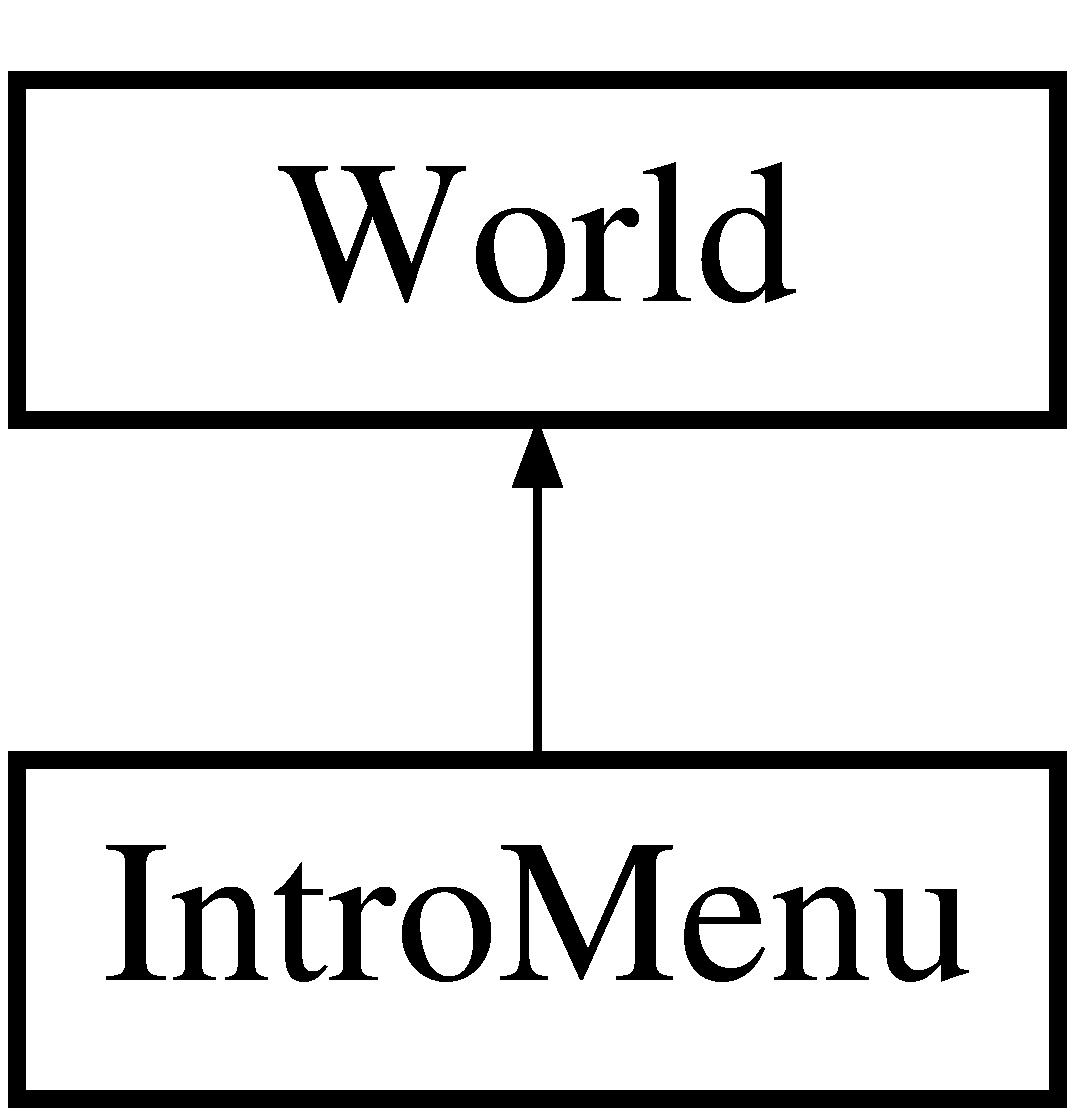
\includegraphics[height=2.000000cm]{class_world}
\end{center}
\end{figure}
\subsection*{Public Member Functions}
\begin{DoxyCompactItemize}
\item 
\hyperlink{class_world_afa39d4e6f714a7a3691ac0c656f5e8a8}{World} ()
\item 
void \hyperlink{class_world_ad76a5c30fcb5d5bbdf0fa7d841b7fb28}{move\-Player} (char direction, \hyperlink{class_player}{Player} $\ast$p)
\item 
void \hyperlink{class_world_a5fc3eeeccb6be52aed487e60fd482bd4}{fire\-Bullet} (\hyperlink{class_player}{Player} $\ast$p)
\item 
bool \hyperlink{class_world_a4c1cbe120ce27ad9e07699805d2d1c2a}{update\-Bullet} ()
\item 
void \hyperlink{class_world_a272362ddd8e710fc99837a5bb7e75c92}{spawn\-Enemy} ()
\item 
bool \hyperlink{class_world_a2fc9351f4b946d4298c6e0dd8337202f}{update\-Enemy} ()
\item 
unsigned int \hyperlink{class_world_acb0800fa65e5a982f79be1caaff4c959}{get\-Enemy\-List\-Size} ()
\item 
unsigned int \hyperlink{class_world_a413a2e1f7353dadff0cec27e92c6a9fe}{get\-Spawn\-Rate} ()
\item 
bool \hyperlink{class_world_a086144235159c3747b099d57d2eff24a}{get\-Refresh} ()
\item 
void \hyperlink{class_world_a4c6b92ca6d00f977710c458ece504aef}{update\-Score} (int add\-To\-Score)
\item 
void \hyperlink{class_world_a9e7ce8f6ae1fff3640cc99cf2f19d54a}{check\-Score} ()
\item 
void \hyperlink{class_world_a6438283b3088d3afe058df7566e7b8e8}{update\-High\-Scores} (\hyperlink{class_player}{Player} $\ast$p)
\item 
void \hyperlink{class_world_af29bd7e1630114caf6f99b2bcd37a647}{show\-High\-Scores} ()
\item 
void \hyperlink{class_world_af75a7049215d511aa08cd568983099e0}{show\-Player\-Lives} (\hyperlink{class_player}{Player} $\ast$p)
\item 
bool \hyperlink{class_world_a1a93b6985e00fc5eb7c417f703332532}{check\-Player\-Lives} (\hyperlink{class_player}{Player} $\ast$p)
\item 
void \hyperlink{class_world_a5ca54d764c1e0305b3110ebffd19fc4d}{check\-Collisions} (\hyperlink{class_player}{Player} $\ast$p)
\begin{DoxyCompactList}\small\item\em -\/--------------------- This is where collision check starts \end{DoxyCompactList}\item 
void \hyperlink{class_world_a4d9747af05b0038a606b30f8e9f66aa3}{update\-Map} (\hyperlink{class_player}{Player} $\ast$p)
\begin{DoxyCompactList}\small\item\em -\/-\/-\/-\/-\/-\/-\/-\/-\/-\/-\/-\/-\/-\/-\/-\/--------------------- End of collision checks \end{DoxyCompactList}\item 
void \hyperlink{class_world_a0656cc8aa64881db8880d6a1af0d5aea}{update\-Display} ()
\item 
bool \hyperlink{class_world_ae5a99f16d3f56792c4c3244b3486db01}{play\-Again} ()
\item 
void \hyperlink{class_world_a642a2e3a23d348ec0166a9ed2fe83272}{play\-Music} (int tune\-I\-D)
\item 
\hyperlink{class_world_a8c73fba541a5817fff65147ba47cd827}{$\sim$\-World} ()
\end{DoxyCompactItemize}
\subsection*{Protected Attributes}
\begin{DoxyCompactItemize}
\item 
char \hyperlink{class_world_abb5635893b4f4c892c4fc034a9950adc}{map} \mbox{[}20\mbox{]}\mbox{[}60\mbox{]}
\item 
\hyperlink{class_sound_f_x_manager}{Sound\-F\-X\-Manager} \hyperlink{class_world_a9985bb370d08feeff87c1d200afe26bc}{sound\-Manager}
\end{DoxyCompactItemize}


\subsection{Detailed Description}


Definition at line 22 of file world.\-h.



\subsection{Constructor \& Destructor Documentation}
\hypertarget{class_world_afa39d4e6f714a7a3691ac0c656f5e8a8}{\index{World@{World}!World@{World}}
\index{World@{World}!World@{World}}
\subsubsection[{World}]{\setlength{\rightskip}{0pt plus 5cm}World\-::\-World (
\begin{DoxyParamCaption}
{}
\end{DoxyParamCaption}
)}}\label{class_world_afa39d4e6f714a7a3691ac0c656f5e8a8}
Load highscores from file

If not loaded, file does not exist so save scores...

If unable to save, there is a problem with the file 

Definition at line 5 of file world.\-cpp.

\hypertarget{class_world_a8c73fba541a5817fff65147ba47cd827}{\index{World@{World}!$\sim$\-World@{$\sim$\-World}}
\index{$\sim$\-World@{$\sim$\-World}!World@{World}}
\subsubsection[{$\sim$\-World}]{\setlength{\rightskip}{0pt plus 5cm}World\-::$\sim$\-World (
\begin{DoxyParamCaption}
{}
\end{DoxyParamCaption}
)}}\label{class_world_a8c73fba541a5817fff65147ba47cd827}


Definition at line 605 of file world.\-cpp.



\subsection{Member Function Documentation}
\hypertarget{class_world_a5ca54d764c1e0305b3110ebffd19fc4d}{\index{World@{World}!check\-Collisions@{check\-Collisions}}
\index{check\-Collisions@{check\-Collisions}!World@{World}}
\subsubsection[{check\-Collisions}]{\setlength{\rightskip}{0pt plus 5cm}void World\-::check\-Collisions (
\begin{DoxyParamCaption}
\item[{{\bf Player} $\ast$}]{p}
\end{DoxyParamCaption}
)}}\label{class_world_a5ca54d764c1e0305b3110ebffd19fc4d}


-\/--------------------- This is where collision check starts 

Temporary locations

Check player location against walls

If player = wall...

Set players location to previous loc

Run through enemy list

Store enemy location in temp loc

Check enemy locations against player

If enemy loc = player loc...

Reset player loc

Decrease lives by 1

Play 'lifelost' sound

Check enemy locations against walls

If enemy = wall...

Store the previous location

Clear the previous location

Delete enemy

Erase entry from the vector list

Update score

Run through bullet list

Store bullet location in temp loc

Check player location against bullets

If player = bullet...

Store the previous location

Clear the previous location

Delete bullet

Remove entry from vector list

Run through enemy list again for each bullet

... (very inefficient)

Store enemy location in temp loc

Check bullet locations against enemies

If bullet = enemy...

Store the previous location

Clear the previous location

Delete enemy

Remove entry from vector list

Update score

Store the previous location

Clear the previous location

Delete bullet

Remove entry from vector list

Play sound

Check bullet locations against walls

If bullet = wall...

Store the previous location

Clear the previous location

Delete bullet

Remove entry from vector list 

Definition at line 100 of file world.\-cpp.

\hypertarget{class_world_a1a93b6985e00fc5eb7c417f703332532}{\index{World@{World}!check\-Player\-Lives@{check\-Player\-Lives}}
\index{check\-Player\-Lives@{check\-Player\-Lives}!World@{World}}
\subsubsection[{check\-Player\-Lives}]{\setlength{\rightskip}{0pt plus 5cm}bool World\-::check\-Player\-Lives (
\begin{DoxyParamCaption}
\item[{{\bf Player} $\ast$}]{p}
\end{DoxyParamCaption}
)}}\label{class_world_a1a93b6985e00fc5eb7c417f703332532}
Get lives

If no lives are left

Stop music

Play 'end game' sound

Otherwise... 

Definition at line 394 of file world.\-cpp.

\hypertarget{class_world_a9e7ce8f6ae1fff3640cc99cf2f19d54a}{\index{World@{World}!check\-Score@{check\-Score}}
\index{check\-Score@{check\-Score}!World@{World}}
\subsubsection[{check\-Score}]{\setlength{\rightskip}{0pt plus 5cm}void World\-::check\-Score (
\begin{DoxyParamCaption}
{}
\end{DoxyParamCaption}
)}}\label{class_world_a9e7ce8f6ae1fff3640cc99cf2f19d54a}


Definition at line 316 of file world.\-cpp.

\hypertarget{class_world_a5fc3eeeccb6be52aed487e60fd482bd4}{\index{World@{World}!fire\-Bullet@{fire\-Bullet}}
\index{fire\-Bullet@{fire\-Bullet}!World@{World}}
\subsubsection[{fire\-Bullet}]{\setlength{\rightskip}{0pt plus 5cm}void World\-::fire\-Bullet (
\begin{DoxyParamCaption}
\item[{{\bf Player} $\ast$}]{p}
\end{DoxyParamCaption}
)}}\label{class_world_a5fc3eeeccb6be52aed487e60fd482bd4}
Instantiate the bullet

Temp location

Store player location

Advance the x position

Set the bullet location

Draw the bullet on the map

Store the bullet in the bullet list

Play 'bullet fired' sound 

Definition at line 3 of file world\-\_\-bullet.\-cpp.

\hypertarget{class_world_acb0800fa65e5a982f79be1caaff4c959}{\index{World@{World}!get\-Enemy\-List\-Size@{get\-Enemy\-List\-Size}}
\index{get\-Enemy\-List\-Size@{get\-Enemy\-List\-Size}!World@{World}}
\subsubsection[{get\-Enemy\-List\-Size}]{\setlength{\rightskip}{0pt plus 5cm}unsigned int World\-::get\-Enemy\-List\-Size (
\begin{DoxyParamCaption}
{}
\end{DoxyParamCaption}
)\hspace{0.3cm}{\ttfamily [inline]}}}\label{class_world_acb0800fa65e5a982f79be1caaff4c959}


Definition at line 54 of file world.\-h.

\hypertarget{class_world_a086144235159c3747b099d57d2eff24a}{\index{World@{World}!get\-Refresh@{get\-Refresh}}
\index{get\-Refresh@{get\-Refresh}!World@{World}}
\subsubsection[{get\-Refresh}]{\setlength{\rightskip}{0pt plus 5cm}bool World\-::get\-Refresh (
\begin{DoxyParamCaption}
{}
\end{DoxyParamCaption}
)\hspace{0.3cm}{\ttfamily [inline]}}}\label{class_world_a086144235159c3747b099d57d2eff24a}


Definition at line 58 of file world.\-h.

\hypertarget{class_world_a413a2e1f7353dadff0cec27e92c6a9fe}{\index{World@{World}!get\-Spawn\-Rate@{get\-Spawn\-Rate}}
\index{get\-Spawn\-Rate@{get\-Spawn\-Rate}!World@{World}}
\subsubsection[{get\-Spawn\-Rate}]{\setlength{\rightskip}{0pt plus 5cm}unsigned int World\-::get\-Spawn\-Rate (
\begin{DoxyParamCaption}
{}
\end{DoxyParamCaption}
)\hspace{0.3cm}{\ttfamily [inline]}}}\label{class_world_a413a2e1f7353dadff0cec27e92c6a9fe}


Definition at line 56 of file world.\-h.

\hypertarget{class_world_ad76a5c30fcb5d5bbdf0fa7d841b7fb28}{\index{World@{World}!move\-Player@{move\-Player}}
\index{move\-Player@{move\-Player}!World@{World}}
\subsubsection[{move\-Player}]{\setlength{\rightskip}{0pt plus 5cm}void World\-::move\-Player (
\begin{DoxyParamCaption}
\item[{char}]{direction, }
\item[{{\bf Player} $\ast$}]{p}
\end{DoxyParamCaption}
)}}\label{class_world_ad76a5c30fcb5d5bbdf0fa7d841b7fb28}
Temp location

Get the current location

Determine direction of travel and adjust the new postion accordingly

Update the position of player 

Definition at line 70 of file world.\-cpp.

\hypertarget{class_world_ae5a99f16d3f56792c4c3244b3486db01}{\index{World@{World}!play\-Again@{play\-Again}}
\index{play\-Again@{play\-Again}!World@{World}}
\subsubsection[{play\-Again}]{\setlength{\rightskip}{0pt plus 5cm}bool World\-::play\-Again (
\begin{DoxyParamCaption}
{}
\end{DoxyParamCaption}
)}}\label{class_world_ae5a99f16d3f56792c4c3244b3486db01}
Message \char`\"{}window\char`\"{} in char array

Run through array

Loop stops before end line char to preserve map edges. 

Definition at line 558 of file world.\-cpp.

\hypertarget{class_world_a642a2e3a23d348ec0166a9ed2fe83272}{\index{World@{World}!play\-Music@{play\-Music}}
\index{play\-Music@{play\-Music}!World@{World}}
\subsubsection[{play\-Music}]{\setlength{\rightskip}{0pt plus 5cm}void World\-::play\-Music (
\begin{DoxyParamCaption}
\item[{int}]{tune\-I\-D}
\end{DoxyParamCaption}
)\hspace{0.3cm}{\ttfamily [inline]}}}\label{class_world_a642a2e3a23d348ec0166a9ed2fe83272}


Definition at line 78 of file world.\-h.

\hypertarget{class_world_af29bd7e1630114caf6f99b2bcd37a647}{\index{World@{World}!show\-High\-Scores@{show\-High\-Scores}}
\index{show\-High\-Scores@{show\-High\-Scores}!World@{World}}
\subsubsection[{show\-High\-Scores}]{\setlength{\rightskip}{0pt plus 5cm}void World\-::show\-High\-Scores (
\begin{DoxyParamCaption}
{}
\end{DoxyParamCaption}
)}}\label{class_world_af29bd7e1630114caf6f99b2bcd37a647}
Temporary high score table

Fills table with high scores from score\-System

Fills map with whole high score table

Clear the highscores from the map 

Definition at line 489 of file world.\-cpp.

\hypertarget{class_world_af75a7049215d511aa08cd568983099e0}{\index{World@{World}!show\-Player\-Lives@{show\-Player\-Lives}}
\index{show\-Player\-Lives@{show\-Player\-Lives}!World@{World}}
\subsubsection[{show\-Player\-Lives}]{\setlength{\rightskip}{0pt plus 5cm}void World\-::show\-Player\-Lives (
\begin{DoxyParamCaption}
\item[{{\bf Player} $\ast$}]{p}
\end{DoxyParamCaption}
)}}\label{class_world_af75a7049215d511aa08cd568983099e0}
Get the lives

Clear previous lives on map

Print lives on map 

Definition at line 375 of file world.\-cpp.

\hypertarget{class_world_a272362ddd8e710fc99837a5bb7e75c92}{\index{World@{World}!spawn\-Enemy@{spawn\-Enemy}}
\index{spawn\-Enemy@{spawn\-Enemy}!World@{World}}
\subsubsection[{spawn\-Enemy}]{\setlength{\rightskip}{0pt plus 5cm}void World\-::spawn\-Enemy (
\begin{DoxyParamCaption}
{}
\end{DoxyParamCaption}
)}}\label{class_world_a272362ddd8e710fc99837a5bb7e75c92}
Instantiate the enemy

Temp location

Set the x coordinate to beside the right wall

Set the y coordinate to a random number between the top and bottom walls.

Extra range check to cut out bad access errors

While random number is N\-O\-T in range

Request another random number

Set the number to the y coordinate

Set the enemy location

Draw the enemy on the map

Store the enemy in the enemy list 

Definition at line 3 of file world\-\_\-enemy.\-cpp.

\hypertarget{class_world_a4c1cbe120ce27ad9e07699805d2d1c2a}{\index{World@{World}!update\-Bullet@{update\-Bullet}}
\index{update\-Bullet@{update\-Bullet}!World@{World}}
\subsubsection[{update\-Bullet}]{\setlength{\rightskip}{0pt plus 5cm}bool World\-::update\-Bullet (
\begin{DoxyParamCaption}
{}
\end{DoxyParamCaption}
)}}\label{class_world_a4c1cbe120ce27ad9e07699805d2d1c2a}
Run through the vector of bullets

Temp location

Get the current location

Advance the proposed location

Set the location

If the vector is not empty return true 

Definition at line 33 of file world\-\_\-bullet.\-cpp.

\hypertarget{class_world_a0656cc8aa64881db8880d6a1af0d5aea}{\index{World@{World}!update\-Display@{update\-Display}}
\index{update\-Display@{update\-Display}!World@{World}}
\subsubsection[{update\-Display}]{\setlength{\rightskip}{0pt plus 5cm}void World\-::update\-Display (
\begin{DoxyParamCaption}
{}
\end{DoxyParamCaption}
)}}\label{class_world_a0656cc8aa64881db8880d6a1af0d5aea}


Definition at line 275 of file world.\-cpp.

\hypertarget{class_world_a2fc9351f4b946d4298c6e0dd8337202f}{\index{World@{World}!update\-Enemy@{update\-Enemy}}
\index{update\-Enemy@{update\-Enemy}!World@{World}}
\subsubsection[{update\-Enemy}]{\setlength{\rightskip}{0pt plus 5cm}bool World\-::update\-Enemy (
\begin{DoxyParamCaption}
{}
\end{DoxyParamCaption}
)}}\label{class_world_a2fc9351f4b946d4298c6e0dd8337202f}
Run through vector of enemies

Temp location

Get the current location

Advance the proposed location

Set the location

If vector is not empty return true 

Definition at line 46 of file world\-\_\-enemy.\-cpp.

\hypertarget{class_world_a6438283b3088d3afe058df7566e7b8e8}{\index{World@{World}!update\-High\-Scores@{update\-High\-Scores}}
\index{update\-High\-Scores@{update\-High\-Scores}!World@{World}}
\subsubsection[{update\-High\-Scores}]{\setlength{\rightskip}{0pt plus 5cm}void World\-::update\-High\-Scores (
\begin{DoxyParamCaption}
\item[{{\bf Player} $\ast$}]{p}
\end{DoxyParamCaption}
)}}\label{class_world_a6438283b3088d3afe058df7566e7b8e8}
Temp initials and score

Store the players current score

Store rank 10's score

Check if the high score has been beaten

Not beaten, exit function

Message \char`\"{}window\char`\"{} in char array

Run through array

Loop stops before end line char to preserve map edges.

Put the score in the high scores

Save highscores 

Definition at line 415 of file world.\-cpp.

\hypertarget{class_world_a4d9747af05b0038a606b30f8e9f66aa3}{\index{World@{World}!update\-Map@{update\-Map}}
\index{update\-Map@{update\-Map}!World@{World}}
\subsubsection[{update\-Map}]{\setlength{\rightskip}{0pt plus 5cm}void World\-::update\-Map (
\begin{DoxyParamCaption}
\item[{{\bf Player} $\ast$}]{p}
\end{DoxyParamCaption}
)}}\label{class_world_a4d9747af05b0038a606b30f8e9f66aa3}


-\/-\/-\/-\/-\/-\/-\/-\/-\/-\/-\/-\/-\/-\/-\/-\/--------------------- End of collision checks 

Store players locations

Draw player on map and clear previous location

Store bullet location

Draw bullet on map and clear previous location

Store enemy location

Draw enemy on map and clear previous location 

Definition at line 245 of file world.\-cpp.

\hypertarget{class_world_a4c6b92ca6d00f977710c458ece504aef}{\index{World@{World}!update\-Score@{update\-Score}}
\index{update\-Score@{update\-Score}!World@{World}}
\subsubsection[{update\-Score}]{\setlength{\rightskip}{0pt plus 5cm}void World\-::update\-Score (
\begin{DoxyParamCaption}
\item[{int}]{add\-To\-Score}
\end{DoxyParamCaption}
)}}\label{class_world_a4c6b92ca6d00f977710c458ece504aef}
Temp score

Get the current score

Add the points to the score

Set the new score

Temp char array to hold text score

Print score from scoring system into array

Update score on map 

Definition at line 289 of file world.\-cpp.



\subsection{Member Data Documentation}
\hypertarget{class_world_abb5635893b4f4c892c4fc034a9950adc}{\index{World@{World}!map@{map}}
\index{map@{map}!World@{World}}
\subsubsection[{map}]{\setlength{\rightskip}{0pt plus 5cm}char World\-::map\mbox{[}20\mbox{]}\mbox{[}60\mbox{]}\hspace{0.3cm}{\ttfamily [protected]}}}\label{class_world_abb5635893b4f4c892c4fc034a9950adc}


Definition at line 39 of file world.\-h.

\hypertarget{class_world_a9985bb370d08feeff87c1d200afe26bc}{\index{World@{World}!sound\-Manager@{sound\-Manager}}
\index{sound\-Manager@{sound\-Manager}!World@{World}}
\subsubsection[{sound\-Manager}]{\setlength{\rightskip}{0pt plus 5cm}{\bf Sound\-F\-X\-Manager} World\-::sound\-Manager\hspace{0.3cm}{\ttfamily [protected]}}}\label{class_world_a9985bb370d08feeff87c1d200afe26bc}


Definition at line 41 of file world.\-h.



The documentation for this class was generated from the following files\-:\begin{DoxyCompactItemize}
\item 
C\-:/\-Users/\-Clarke/\-Documents/\-Codeblocks/\-O\-Omap\-Game/include/\hyperlink{world_8h}{world.\-h}\item 
C\-:/\-Users/\-Clarke/\-Documents/\-Codeblocks/\-O\-Omap\-Game/src/\hyperlink{world_8cpp}{world.\-cpp}\item 
C\-:/\-Users/\-Clarke/\-Documents/\-Codeblocks/\-O\-Omap\-Game/\hyperlink{world__bullet_8cpp}{world\-\_\-bullet.\-cpp}\item 
C\-:/\-Users/\-Clarke/\-Documents/\-Codeblocks/\-O\-Omap\-Game/\hyperlink{world__enemy_8cpp}{world\-\_\-enemy.\-cpp}\end{DoxyCompactItemize}

\chapter{File Documentation}
\hypertarget{bullet_8h}{\section{C\-:/\-Users/\-Clarke/\-Documents/\-Codeblocks/\-O\-Omap\-Game/include/bullet.h File Reference}
\label{bullet_8h}\index{C\-:/\-Users/\-Clarke/\-Documents/\-Codeblocks/\-O\-Omap\-Game/include/bullet.\-h@{C\-:/\-Users/\-Clarke/\-Documents/\-Codeblocks/\-O\-Omap\-Game/include/bullet.\-h}}
}
{\ttfamily \#include \char`\"{}C\-:/\-Users/\-Clarke/\-Documents/\-Codeblocks/\-O\-Omap\-Game/resources.\-h\char`\"{}}\\*
\subsection*{Classes}
\begin{DoxyCompactItemize}
\item 
class \hyperlink{class_bullet}{Bullet}
\end{DoxyCompactItemize}

\hypertarget{enemy_8h}{\section{C\-:/\-Users/\-Clarke/\-Documents/\-Codeblocks/\-O\-Omap\-Game/include/enemy.h File Reference}
\label{enemy_8h}\index{C\-:/\-Users/\-Clarke/\-Documents/\-Codeblocks/\-O\-Omap\-Game/include/enemy.\-h@{C\-:/\-Users/\-Clarke/\-Documents/\-Codeblocks/\-O\-Omap\-Game/include/enemy.\-h}}
}
{\ttfamily \#include \char`\"{}C\-:/\-Users/\-Clarke/\-Documents/\-Codeblocks/\-O\-Omap\-Game/resources.\-h\char`\"{}}\\*
\subsection*{Classes}
\begin{DoxyCompactItemize}
\item 
class \hyperlink{class_enemy}{Enemy}
\end{DoxyCompactItemize}

\hypertarget{intromenu_8h}{\section{C\-:/\-Users/\-Clarke/\-Documents/\-Codeblocks/\-O\-Omap\-Game/include/intromenu.h File Reference}
\label{intromenu_8h}\index{C\-:/\-Users/\-Clarke/\-Documents/\-Codeblocks/\-O\-Omap\-Game/include/intromenu.\-h@{C\-:/\-Users/\-Clarke/\-Documents/\-Codeblocks/\-O\-Omap\-Game/include/intromenu.\-h}}
}
{\ttfamily \#include \char`\"{}windows.\-h\char`\"{}}\\*
{\ttfamily \#include \char`\"{}world.\-h\char`\"{}}\\*
\subsection*{Classes}
\begin{DoxyCompactItemize}
\item 
class \hyperlink{class_intro_menu}{Intro\-Menu}
\end{DoxyCompactItemize}

\hypertarget{intromessage_8h}{\section{C\-:/\-Users/\-Clarke/\-Documents/\-Codeblocks/\-O\-Omap\-Game/include/intromessage.h File Reference}
\label{intromessage_8h}\index{C\-:/\-Users/\-Clarke/\-Documents/\-Codeblocks/\-O\-Omap\-Game/include/intromessage.\-h@{C\-:/\-Users/\-Clarke/\-Documents/\-Codeblocks/\-O\-Omap\-Game/include/intromessage.\-h}}
}
{\ttfamily \#include \char`\"{}resources.\-h\char`\"{}}\\*
\subsection*{Classes}
\begin{DoxyCompactItemize}
\item 
class \hyperlink{classintromessage}{intromessage}
\end{DoxyCompactItemize}

\hypertarget{player_8h}{\section{C\-:/\-Users/\-Clarke/\-Documents/\-Codeblocks/\-O\-Omap\-Game/include/player.h File Reference}
\label{player_8h}\index{C\-:/\-Users/\-Clarke/\-Documents/\-Codeblocks/\-O\-Omap\-Game/include/player.\-h@{C\-:/\-Users/\-Clarke/\-Documents/\-Codeblocks/\-O\-Omap\-Game/include/player.\-h}}
}
{\ttfamily \#include \char`\"{}C\-:/\-Users/\-Clarke/\-Documents/\-Codeblocks/\-O\-Omap\-Game/resources.\-h\char`\"{}}\\*
\subsection*{Classes}
\begin{DoxyCompactItemize}
\item 
class \hyperlink{class_player}{Player}
\end{DoxyCompactItemize}

\hypertarget{scoring_8h}{\section{C\-:/\-Users/\-Clarke/\-Documents/\-Codeblocks/\-O\-Omap\-Game/include/scoring.h File Reference}
\label{scoring_8h}\index{C\-:/\-Users/\-Clarke/\-Documents/\-Codeblocks/\-O\-Omap\-Game/include/scoring.\-h@{C\-:/\-Users/\-Clarke/\-Documents/\-Codeblocks/\-O\-Omap\-Game/include/scoring.\-h}}
}
{\ttfamily \#include $<$iostream$>$}\\*
{\ttfamily \#include $<$fstream$>$}\\*
{\ttfamily \#include \char`\"{}C\-:/\-Users/\-Clarke/\-Documents/\-Codeblocks/\-O\-Omap\-Game/resources.\-h\char`\"{}}\\*
\subsection*{Classes}
\begin{DoxyCompactItemize}
\item 
class \hyperlink{class_scoring}{Scoring}
\end{DoxyCompactItemize}

\hypertarget{soundmanager_8h}{\section{C\-:/\-Users/\-Clarke/\-Documents/\-Codeblocks/\-O\-Omap\-Game/include/soundmanager.h File Reference}
\label{soundmanager_8h}\index{C\-:/\-Users/\-Clarke/\-Documents/\-Codeblocks/\-O\-Omap\-Game/include/soundmanager.\-h@{C\-:/\-Users/\-Clarke/\-Documents/\-Codeblocks/\-O\-Omap\-Game/include/soundmanager.\-h}}
}
{\ttfamily \#include $<$iostream$>$}\\*
{\ttfamily \#include $<$S\-F\-M\-L/\-Audio.\-hpp$>$}\\*
\subsection*{Classes}
\begin{DoxyCompactItemize}
\item 
class \hyperlink{class_sound_f_x_manager}{Sound\-F\-X\-Manager}
\end{DoxyCompactItemize}
\subsection*{Enumerations}
\begin{DoxyCompactItemize}
\item 
enum \{ \\*
\hyperlink{soundmanager_8h_a06fc87d81c62e9abb8790b6e5713c55ba4173ed5086ea390fbfe53dcfe32cdb64}{S\-O\-U\-N\-D\-\_\-\-B\-E\-G\-I\-N} = 0, 
\hyperlink{soundmanager_8h_a06fc87d81c62e9abb8790b6e5713c55bae905da11e28c818b965c0d5d25ca4559}{S\-O\-U\-N\-D\-\_\-\-F\-I\-R\-E}, 
\hyperlink{soundmanager_8h_a06fc87d81c62e9abb8790b6e5713c55bac34f4788f6453a436988c1770809b524}{S\-O\-U\-N\-D\-\_\-\-L\-O\-S\-E\-L\-I\-F\-E}, 
\hyperlink{soundmanager_8h_a06fc87d81c62e9abb8790b6e5713c55bada17f93576300ab9149bbdd9151760fe}{S\-O\-U\-N\-D\-\_\-\-E\-N\-E\-M\-Y\-D\-E\-A\-D}, 
\\*
\hyperlink{soundmanager_8h_a06fc87d81c62e9abb8790b6e5713c55baf5be469dd36445d8f37d631a83528c49}{S\-O\-U\-N\-D\-\_\-\-S\-E\-L\-E\-C\-T}, 
\hyperlink{soundmanager_8h_a06fc87d81c62e9abb8790b6e5713c55ba9e538a66e793e0146dfd59ae05b5e030}{S\-O\-U\-N\-D\-\_\-\-E\-N\-D\-G\-A\-M\-E}
 \}
\end{DoxyCompactItemize}


\subsection{Enumeration Type Documentation}
\hypertarget{soundmanager_8h_a06fc87d81c62e9abb8790b6e5713c55b}{\subsubsection[{anonymous enum}]{\setlength{\rightskip}{0pt plus 5cm}anonymous enum}}\label{soundmanager_8h_a06fc87d81c62e9abb8790b6e5713c55b}
\begin{Desc}
\item[Enumerator]\par
\begin{description}
\index{S\-O\-U\-N\-D\-\_\-\-B\-E\-G\-I\-N@{S\-O\-U\-N\-D\-\_\-\-B\-E\-G\-I\-N}!soundmanager.\-h@{soundmanager.\-h}}\index{soundmanager.\-h@{soundmanager.\-h}!S\-O\-U\-N\-D\-\_\-\-B\-E\-G\-I\-N@{S\-O\-U\-N\-D\-\_\-\-B\-E\-G\-I\-N}}\item[{\em 
\hypertarget{soundmanager_8h_a06fc87d81c62e9abb8790b6e5713c55ba4173ed5086ea390fbfe53dcfe32cdb64}{S\-O\-U\-N\-D\-\_\-\-B\-E\-G\-I\-N}\label{soundmanager_8h_a06fc87d81c62e9abb8790b6e5713c55ba4173ed5086ea390fbfe53dcfe32cdb64}
}]\index{S\-O\-U\-N\-D\-\_\-\-F\-I\-R\-E@{S\-O\-U\-N\-D\-\_\-\-F\-I\-R\-E}!soundmanager.\-h@{soundmanager.\-h}}\index{soundmanager.\-h@{soundmanager.\-h}!S\-O\-U\-N\-D\-\_\-\-F\-I\-R\-E@{S\-O\-U\-N\-D\-\_\-\-F\-I\-R\-E}}\item[{\em 
\hypertarget{soundmanager_8h_a06fc87d81c62e9abb8790b6e5713c55bae905da11e28c818b965c0d5d25ca4559}{S\-O\-U\-N\-D\-\_\-\-F\-I\-R\-E}\label{soundmanager_8h_a06fc87d81c62e9abb8790b6e5713c55bae905da11e28c818b965c0d5d25ca4559}
}]\index{S\-O\-U\-N\-D\-\_\-\-L\-O\-S\-E\-L\-I\-F\-E@{S\-O\-U\-N\-D\-\_\-\-L\-O\-S\-E\-L\-I\-F\-E}!soundmanager.\-h@{soundmanager.\-h}}\index{soundmanager.\-h@{soundmanager.\-h}!S\-O\-U\-N\-D\-\_\-\-L\-O\-S\-E\-L\-I\-F\-E@{S\-O\-U\-N\-D\-\_\-\-L\-O\-S\-E\-L\-I\-F\-E}}\item[{\em 
\hypertarget{soundmanager_8h_a06fc87d81c62e9abb8790b6e5713c55bac34f4788f6453a436988c1770809b524}{S\-O\-U\-N\-D\-\_\-\-L\-O\-S\-E\-L\-I\-F\-E}\label{soundmanager_8h_a06fc87d81c62e9abb8790b6e5713c55bac34f4788f6453a436988c1770809b524}
}]\index{S\-O\-U\-N\-D\-\_\-\-E\-N\-E\-M\-Y\-D\-E\-A\-D@{S\-O\-U\-N\-D\-\_\-\-E\-N\-E\-M\-Y\-D\-E\-A\-D}!soundmanager.\-h@{soundmanager.\-h}}\index{soundmanager.\-h@{soundmanager.\-h}!S\-O\-U\-N\-D\-\_\-\-E\-N\-E\-M\-Y\-D\-E\-A\-D@{S\-O\-U\-N\-D\-\_\-\-E\-N\-E\-M\-Y\-D\-E\-A\-D}}\item[{\em 
\hypertarget{soundmanager_8h_a06fc87d81c62e9abb8790b6e5713c55bada17f93576300ab9149bbdd9151760fe}{S\-O\-U\-N\-D\-\_\-\-E\-N\-E\-M\-Y\-D\-E\-A\-D}\label{soundmanager_8h_a06fc87d81c62e9abb8790b6e5713c55bada17f93576300ab9149bbdd9151760fe}
}]\index{S\-O\-U\-N\-D\-\_\-\-S\-E\-L\-E\-C\-T@{S\-O\-U\-N\-D\-\_\-\-S\-E\-L\-E\-C\-T}!soundmanager.\-h@{soundmanager.\-h}}\index{soundmanager.\-h@{soundmanager.\-h}!S\-O\-U\-N\-D\-\_\-\-S\-E\-L\-E\-C\-T@{S\-O\-U\-N\-D\-\_\-\-S\-E\-L\-E\-C\-T}}\item[{\em 
\hypertarget{soundmanager_8h_a06fc87d81c62e9abb8790b6e5713c55baf5be469dd36445d8f37d631a83528c49}{S\-O\-U\-N\-D\-\_\-\-S\-E\-L\-E\-C\-T}\label{soundmanager_8h_a06fc87d81c62e9abb8790b6e5713c55baf5be469dd36445d8f37d631a83528c49}
}]\index{S\-O\-U\-N\-D\-\_\-\-E\-N\-D\-G\-A\-M\-E@{S\-O\-U\-N\-D\-\_\-\-E\-N\-D\-G\-A\-M\-E}!soundmanager.\-h@{soundmanager.\-h}}\index{soundmanager.\-h@{soundmanager.\-h}!S\-O\-U\-N\-D\-\_\-\-E\-N\-D\-G\-A\-M\-E@{S\-O\-U\-N\-D\-\_\-\-E\-N\-D\-G\-A\-M\-E}}\item[{\em 
\hypertarget{soundmanager_8h_a06fc87d81c62e9abb8790b6e5713c55ba9e538a66e793e0146dfd59ae05b5e030}{S\-O\-U\-N\-D\-\_\-\-E\-N\-D\-G\-A\-M\-E}\label{soundmanager_8h_a06fc87d81c62e9abb8790b6e5713c55ba9e538a66e793e0146dfd59ae05b5e030}
}]\end{description}
\end{Desc}


Definition at line 9 of file soundmanager.\-h.


\hypertarget{world_8h}{\section{C\-:/\-Users/\-Clarke/\-Documents/\-Codeblocks/\-O\-Omap\-Game/include/world.h File Reference}
\label{world_8h}\index{C\-:/\-Users/\-Clarke/\-Documents/\-Codeblocks/\-O\-Omap\-Game/include/world.\-h@{C\-:/\-Users/\-Clarke/\-Documents/\-Codeblocks/\-O\-Omap\-Game/include/world.\-h}}
}
{\ttfamily \#include $<$iostream$>$}\\*
{\ttfamily \#include $<$vector$>$}\\*
{\ttfamily \#include $<$sstream$>$}\\*
{\ttfamily \#include \char`\"{}stdio.\-h\char`\"{}}\\*
{\ttfamily \#include \char`\"{}windows.\-h\char`\"{}}\\*
{\ttfamily \#include \char`\"{}time.\-h\char`\"{}}\\*
{\ttfamily \#include \char`\"{}C\-:/\-Users/\-Clarke/\-Documents/\-Codeblocks/\-O\-Omap\-Game/resources.\-h\char`\"{}}\\*
{\ttfamily \#include \char`\"{}player.\-h\char`\"{}}\\*
{\ttfamily \#include \char`\"{}bullet.\-h\char`\"{}}\\*
{\ttfamily \#include \char`\"{}enemy.\-h\char`\"{}}\\*
{\ttfamily \#include \char`\"{}scoring.\-h\char`\"{}}\\*
{\ttfamily \#include \char`\"{}soundmanager.\-h\char`\"{}}\\*
\subsection*{Classes}
\begin{DoxyCompactItemize}
\item 
class \hyperlink{class_world}{World}
\end{DoxyCompactItemize}
\subsection*{Macros}
\begin{DoxyCompactItemize}
\item 
\#define \hyperlink{world_8h_ac50762666aa00bd3a4308158510f1748}{\-\_\-\-W\-I\-N32\-\_\-\-W\-I\-N\-N\-T}~0x0600
\end{DoxyCompactItemize}


\subsection{Macro Definition Documentation}
\hypertarget{world_8h_ac50762666aa00bd3a4308158510f1748}{\index{world.\-h@{world.\-h}!\-\_\-\-W\-I\-N32\-\_\-\-W\-I\-N\-N\-T@{\-\_\-\-W\-I\-N32\-\_\-\-W\-I\-N\-N\-T}}
\index{\-\_\-\-W\-I\-N32\-\_\-\-W\-I\-N\-N\-T@{\-\_\-\-W\-I\-N32\-\_\-\-W\-I\-N\-N\-T}!world.h@{world.\-h}}
\subsubsection[{\-\_\-\-W\-I\-N32\-\_\-\-W\-I\-N\-N\-T}]{\setlength{\rightskip}{0pt plus 5cm}\#define \-\_\-\-W\-I\-N32\-\_\-\-W\-I\-N\-N\-T~0x0600}}\label{world_8h_ac50762666aa00bd3a4308158510f1748}


Definition at line 4 of file world.\-h.


\hypertarget{main_8cpp}{\section{C\-:/\-Users/\-Clarke/\-Documents/\-Codeblocks/\-O\-Omap\-Game/main.cpp File Reference}
\label{main_8cpp}\index{C\-:/\-Users/\-Clarke/\-Documents/\-Codeblocks/\-O\-Omap\-Game/main.\-cpp@{C\-:/\-Users/\-Clarke/\-Documents/\-Codeblocks/\-O\-Omap\-Game/main.\-cpp}}
}
{\ttfamily \#include $<$iostream$>$}\\*
{\ttfamily \#include \char`\"{}windows.\-h\char`\"{}}\\*
{\ttfamily \#include \char`\"{}C\-:/\-Users/\-Clarke/\-Documents/\-Codeblocks/\-O\-Omap\-Game/include/world.\-h\char`\"{}}\\*
{\ttfamily \#include \char`\"{}C\-:/\-Users/\-Clarke/\-Documents/\-Codeblocks/\-O\-Omap\-Game/include/intromenu.\-h\char`\"{}}\\*
{\ttfamily \#include \char`\"{}resources.\-h\char`\"{}}\\*
\subsection*{Functions}
\begin{DoxyCompactItemize}
\item 
int \hyperlink{main_8cpp_ae66f6b31b5ad750f1fe042a706a4e3d4}{main} ()
\end{DoxyCompactItemize}


\subsection{Function Documentation}
\hypertarget{main_8cpp_ae66f6b31b5ad750f1fe042a706a4e3d4}{\index{main.\-cpp@{main.\-cpp}!main@{main}}
\index{main@{main}!main.cpp@{main.\-cpp}}
\subsubsection[{main}]{\setlength{\rightskip}{0pt plus 5cm}int main (
\begin{DoxyParamCaption}
{}
\end{DoxyParamCaption}
)}}\label{main_8cpp_ae66f6b31b5ad750f1fe042a706a4e3d4}
Create an intro instance

Create world instance

Create a \hyperlink{class_player}{Player} instance

Display the title screen

Display the introduction message

Update the map

Show the display

Play music

Start of game loop

Increment the loop counter

Reset direction

Arrow key down

Arrow key up

Arrow key right

Arrow key left

Arrow key up/left

Arrow key up/right

Arrow key down/right

Arrow key down/left

Fire a bullet giving the address of plyr1 to get their location

Check the score This adjusts the spawn rate too

Set spawn rate

S\-P\-A\-W\-N E\-N\-E\-M\-Y If the counter is over the spawn rate

Spawn an ememy

Reset the loop counter

U\-P\-D\-A\-T\-E E\-N\-E\-M\-Y Update any enemy's position setting refresh to true if enemies are present

F\-I\-R\-E B\-U\-L\-L\-E\-T\-S Update position of bullets setting refresh to true if bullets are there

Direction If a direction has been pressed or a bullet has been fired or enemies are present

If player has moved

Move player

Check collisions

Update map

Update lives

Update display

Reset player refresh

Wait 30 milliseconds

Escape to exit

set bool to false to break out of game loop

End of game loop

Display end game message...

Add score to highscores

Show highscores

Ask user to play again

End of play again loop 

Definition at line 20 of file main.\-cpp.


\hypertarget{resources_8cpp}{\section{C\-:/\-Users/\-Clarke/\-Documents/\-Codeblocks/\-O\-Omap\-Game/resources.cpp File Reference}
\label{resources_8cpp}\index{C\-:/\-Users/\-Clarke/\-Documents/\-Codeblocks/\-O\-Omap\-Game/resources.\-cpp@{C\-:/\-Users/\-Clarke/\-Documents/\-Codeblocks/\-O\-Omap\-Game/resources.\-cpp}}
}
{\ttfamily \#include \char`\"{}resources.\-h\char`\"{}}\\*
\subsection*{Functions}
\begin{DoxyCompactItemize}
\item 
void \hyperlink{resources_8cpp_a6a3ca153f0817e8ba91a023b886bb662}{Clear\-Screen} ()
\item 
int \hyperlink{resources_8cpp_aa6006a265ed886e0b70e3324ca908ad4}{Random\-Number} (int minimum, int maximum)
\end{DoxyCompactItemize}


\subsection{Function Documentation}
\hypertarget{resources_8cpp_a6a3ca153f0817e8ba91a023b886bb662}{\index{resources.\-cpp@{resources.\-cpp}!Clear\-Screen@{Clear\-Screen}}
\index{Clear\-Screen@{Clear\-Screen}!resources.cpp@{resources.\-cpp}}
\subsubsection[{Clear\-Screen}]{\setlength{\rightskip}{0pt plus 5cm}void Clear\-Screen (
\begin{DoxyParamCaption}
{}
\end{DoxyParamCaption}
)}}\label{resources_8cpp_a6a3ca153f0817e8ba91a023b886bb662}


Definition at line 3 of file resources.\-cpp.

\hypertarget{resources_8cpp_aa6006a265ed886e0b70e3324ca908ad4}{\index{resources.\-cpp@{resources.\-cpp}!Random\-Number@{Random\-Number}}
\index{Random\-Number@{Random\-Number}!resources.cpp@{resources.\-cpp}}
\subsubsection[{Random\-Number}]{\setlength{\rightskip}{0pt plus 5cm}int Random\-Number (
\begin{DoxyParamCaption}
\item[{int}]{minimum, }
\item[{int}]{maximum}
\end{DoxyParamCaption}
)}}\label{resources_8cpp_aa6006a265ed886e0b70e3324ca908ad4}
Create a random seed

Generate random number between min and max 

Definition at line 40 of file resources.\-cpp.


\hypertarget{resources_8h}{\section{C\-:/\-Users/\-Clarke/\-Documents/\-Codeblocks/\-O\-Omap\-Game/resources.h File Reference}
\label{resources_8h}\index{C\-:/\-Users/\-Clarke/\-Documents/\-Codeblocks/\-O\-Omap\-Game/resources.\-h@{C\-:/\-Users/\-Clarke/\-Documents/\-Codeblocks/\-O\-Omap\-Game/resources.\-h}}
}
{\ttfamily \#include \char`\"{}windows.\-h\char`\"{}}\\*
{\ttfamily \#include \char`\"{}stdlib.\-h\char`\"{}}\\*
{\ttfamily \#include \char`\"{}time.\-h\char`\"{}}\\*
\subsection*{Classes}
\begin{DoxyCompactItemize}
\item 
struct \hyperlink{structlocation}{location}
\item 
struct \hyperlink{struct_score}{Score}
\end{DoxyCompactItemize}
\subsection*{Enumerations}
\begin{DoxyCompactItemize}
\item 
enum \hyperlink{resources_8h_a6d8f83e710b27d4f86c45f0bb77066e3}{entity\-\_\-type} \{ \hyperlink{resources_8h_a6d8f83e710b27d4f86c45f0bb77066e3a3d6f42508532cf645d64d561d145bdfc}{E\-N\-T\-I\-T\-Y\-\_\-\-T\-Y\-P\-E\-\_\-\-P\-L\-A\-Y\-E\-R} = 0, 
\hyperlink{resources_8h_a6d8f83e710b27d4f86c45f0bb77066e3aa5c16f3c78d8d998acd8b48fa5be3bab}{E\-N\-T\-I\-T\-Y\-\_\-\-T\-Y\-P\-E\-\_\-\-E\-N\-E\-M\-Y}, 
\hyperlink{resources_8h_a6d8f83e710b27d4f86c45f0bb77066e3a0679eaabbbf032f3306e08cd036990b4}{E\-N\-T\-I\-T\-Y\-\_\-\-T\-Y\-P\-E\-\_\-\-B\-U\-L\-L\-E\-T}
 \}
\item 
enum \hyperlink{resources_8h_a7a678f8ed72ac1adab42d1cf8e4d5b9d}{collision\-\_\-outcome\-\_\-type} \{ \hyperlink{resources_8h_a7a678f8ed72ac1adab42d1cf8e4d5b9da8f2787945cf0007e858252aed3eb18ff}{C\-O\-L\-L\-\_\-\-T\-Y\-P\-E\-\_\-\-N\-O\-\_\-\-C\-O\-L\-L} = 0, 
\hyperlink{resources_8h_a7a678f8ed72ac1adab42d1cf8e4d5b9daec6447a76dd802c99a4a1111861ec9be}{C\-O\-L\-L\-\_\-\-T\-Y\-P\-E\-\_\-\-N\-O\-T\-H\-I\-N\-G}, 
\hyperlink{resources_8h_a7a678f8ed72ac1adab42d1cf8e4d5b9daa35c9ddf0544d4c0008530a32ee4f829}{C\-O\-L\-L\-\_\-\-T\-Y\-P\-E\-\_\-\-D\-E\-A\-D}
 \}
\end{DoxyCompactItemize}
\subsection*{Functions}
\begin{DoxyCompactItemize}
\item 
void \hyperlink{resources_8h_a6a3ca153f0817e8ba91a023b886bb662}{Clear\-Screen} ()
\item 
int \hyperlink{resources_8h_aa6006a265ed886e0b70e3324ca908ad4}{Random\-Number} (int minimum, int maximum)
\end{DoxyCompactItemize}


\subsection{Enumeration Type Documentation}
\hypertarget{resources_8h_a7a678f8ed72ac1adab42d1cf8e4d5b9d}{\index{resources.\-h@{resources.\-h}!collision\-\_\-outcome\-\_\-type@{collision\-\_\-outcome\-\_\-type}}
\index{collision\-\_\-outcome\-\_\-type@{collision\-\_\-outcome\-\_\-type}!resources.h@{resources.\-h}}
\subsubsection[{collision\-\_\-outcome\-\_\-type}]{\setlength{\rightskip}{0pt plus 5cm}enum {\bf collision\-\_\-outcome\-\_\-type}}}\label{resources_8h_a7a678f8ed72ac1adab42d1cf8e4d5b9d}
\begin{Desc}
\item[Enumerator]\par
\begin{description}
\index{C\-O\-L\-L\-\_\-\-T\-Y\-P\-E\-\_\-\-N\-O\-\_\-\-C\-O\-L\-L@{C\-O\-L\-L\-\_\-\-T\-Y\-P\-E\-\_\-\-N\-O\-\_\-\-C\-O\-L\-L}!resources.\-h@{resources.\-h}}\index{resources.\-h@{resources.\-h}!C\-O\-L\-L\-\_\-\-T\-Y\-P\-E\-\_\-\-N\-O\-\_\-\-C\-O\-L\-L@{C\-O\-L\-L\-\_\-\-T\-Y\-P\-E\-\_\-\-N\-O\-\_\-\-C\-O\-L\-L}}\item[{\em 
\hypertarget{resources_8h_a7a678f8ed72ac1adab42d1cf8e4d5b9da8f2787945cf0007e858252aed3eb18ff}{C\-O\-L\-L\-\_\-\-T\-Y\-P\-E\-\_\-\-N\-O\-\_\-\-C\-O\-L\-L}\label{resources_8h_a7a678f8ed72ac1adab42d1cf8e4d5b9da8f2787945cf0007e858252aed3eb18ff}
}]\index{C\-O\-L\-L\-\_\-\-T\-Y\-P\-E\-\_\-\-N\-O\-T\-H\-I\-N\-G@{C\-O\-L\-L\-\_\-\-T\-Y\-P\-E\-\_\-\-N\-O\-T\-H\-I\-N\-G}!resources.\-h@{resources.\-h}}\index{resources.\-h@{resources.\-h}!C\-O\-L\-L\-\_\-\-T\-Y\-P\-E\-\_\-\-N\-O\-T\-H\-I\-N\-G@{C\-O\-L\-L\-\_\-\-T\-Y\-P\-E\-\_\-\-N\-O\-T\-H\-I\-N\-G}}\item[{\em 
\hypertarget{resources_8h_a7a678f8ed72ac1adab42d1cf8e4d5b9daec6447a76dd802c99a4a1111861ec9be}{C\-O\-L\-L\-\_\-\-T\-Y\-P\-E\-\_\-\-N\-O\-T\-H\-I\-N\-G}\label{resources_8h_a7a678f8ed72ac1adab42d1cf8e4d5b9daec6447a76dd802c99a4a1111861ec9be}
}]\index{C\-O\-L\-L\-\_\-\-T\-Y\-P\-E\-\_\-\-D\-E\-A\-D@{C\-O\-L\-L\-\_\-\-T\-Y\-P\-E\-\_\-\-D\-E\-A\-D}!resources.\-h@{resources.\-h}}\index{resources.\-h@{resources.\-h}!C\-O\-L\-L\-\_\-\-T\-Y\-P\-E\-\_\-\-D\-E\-A\-D@{C\-O\-L\-L\-\_\-\-T\-Y\-P\-E\-\_\-\-D\-E\-A\-D}}\item[{\em 
\hypertarget{resources_8h_a7a678f8ed72ac1adab42d1cf8e4d5b9daa35c9ddf0544d4c0008530a32ee4f829}{C\-O\-L\-L\-\_\-\-T\-Y\-P\-E\-\_\-\-D\-E\-A\-D}\label{resources_8h_a7a678f8ed72ac1adab42d1cf8e4d5b9daa35c9ddf0544d4c0008530a32ee4f829}
}]\end{description}
\end{Desc}


Definition at line 23 of file resources.\-h.

\hypertarget{resources_8h_a6d8f83e710b27d4f86c45f0bb77066e3}{\index{resources.\-h@{resources.\-h}!entity\-\_\-type@{entity\-\_\-type}}
\index{entity\-\_\-type@{entity\-\_\-type}!resources.h@{resources.\-h}}
\subsubsection[{entity\-\_\-type}]{\setlength{\rightskip}{0pt plus 5cm}enum {\bf entity\-\_\-type}}}\label{resources_8h_a6d8f83e710b27d4f86c45f0bb77066e3}
\begin{Desc}
\item[Enumerator]\par
\begin{description}
\index{E\-N\-T\-I\-T\-Y\-\_\-\-T\-Y\-P\-E\-\_\-\-P\-L\-A\-Y\-E\-R@{E\-N\-T\-I\-T\-Y\-\_\-\-T\-Y\-P\-E\-\_\-\-P\-L\-A\-Y\-E\-R}!resources.\-h@{resources.\-h}}\index{resources.\-h@{resources.\-h}!E\-N\-T\-I\-T\-Y\-\_\-\-T\-Y\-P\-E\-\_\-\-P\-L\-A\-Y\-E\-R@{E\-N\-T\-I\-T\-Y\-\_\-\-T\-Y\-P\-E\-\_\-\-P\-L\-A\-Y\-E\-R}}\item[{\em 
\hypertarget{resources_8h_a6d8f83e710b27d4f86c45f0bb77066e3a3d6f42508532cf645d64d561d145bdfc}{E\-N\-T\-I\-T\-Y\-\_\-\-T\-Y\-P\-E\-\_\-\-P\-L\-A\-Y\-E\-R}\label{resources_8h_a6d8f83e710b27d4f86c45f0bb77066e3a3d6f42508532cf645d64d561d145bdfc}
}]\index{E\-N\-T\-I\-T\-Y\-\_\-\-T\-Y\-P\-E\-\_\-\-E\-N\-E\-M\-Y@{E\-N\-T\-I\-T\-Y\-\_\-\-T\-Y\-P\-E\-\_\-\-E\-N\-E\-M\-Y}!resources.\-h@{resources.\-h}}\index{resources.\-h@{resources.\-h}!E\-N\-T\-I\-T\-Y\-\_\-\-T\-Y\-P\-E\-\_\-\-E\-N\-E\-M\-Y@{E\-N\-T\-I\-T\-Y\-\_\-\-T\-Y\-P\-E\-\_\-\-E\-N\-E\-M\-Y}}\item[{\em 
\hypertarget{resources_8h_a6d8f83e710b27d4f86c45f0bb77066e3aa5c16f3c78d8d998acd8b48fa5be3bab}{E\-N\-T\-I\-T\-Y\-\_\-\-T\-Y\-P\-E\-\_\-\-E\-N\-E\-M\-Y}\label{resources_8h_a6d8f83e710b27d4f86c45f0bb77066e3aa5c16f3c78d8d998acd8b48fa5be3bab}
}]\index{E\-N\-T\-I\-T\-Y\-\_\-\-T\-Y\-P\-E\-\_\-\-B\-U\-L\-L\-E\-T@{E\-N\-T\-I\-T\-Y\-\_\-\-T\-Y\-P\-E\-\_\-\-B\-U\-L\-L\-E\-T}!resources.\-h@{resources.\-h}}\index{resources.\-h@{resources.\-h}!E\-N\-T\-I\-T\-Y\-\_\-\-T\-Y\-P\-E\-\_\-\-B\-U\-L\-L\-E\-T@{E\-N\-T\-I\-T\-Y\-\_\-\-T\-Y\-P\-E\-\_\-\-B\-U\-L\-L\-E\-T}}\item[{\em 
\hypertarget{resources_8h_a6d8f83e710b27d4f86c45f0bb77066e3a0679eaabbbf032f3306e08cd036990b4}{E\-N\-T\-I\-T\-Y\-\_\-\-T\-Y\-P\-E\-\_\-\-B\-U\-L\-L\-E\-T}\label{resources_8h_a6d8f83e710b27d4f86c45f0bb77066e3a0679eaabbbf032f3306e08cd036990b4}
}]\end{description}
\end{Desc}


Definition at line 13 of file resources.\-h.



\subsection{Function Documentation}
\hypertarget{resources_8h_a6a3ca153f0817e8ba91a023b886bb662}{\index{resources.\-h@{resources.\-h}!Clear\-Screen@{Clear\-Screen}}
\index{Clear\-Screen@{Clear\-Screen}!resources.h@{resources.\-h}}
\subsubsection[{Clear\-Screen}]{\setlength{\rightskip}{0pt plus 5cm}void Clear\-Screen (
\begin{DoxyParamCaption}
{}
\end{DoxyParamCaption}
)}}\label{resources_8h_a6a3ca153f0817e8ba91a023b886bb662}


Definition at line 3 of file resources.\-cpp.

\hypertarget{resources_8h_aa6006a265ed886e0b70e3324ca908ad4}{\index{resources.\-h@{resources.\-h}!Random\-Number@{Random\-Number}}
\index{Random\-Number@{Random\-Number}!resources.h@{resources.\-h}}
\subsubsection[{Random\-Number}]{\setlength{\rightskip}{0pt plus 5cm}int Random\-Number (
\begin{DoxyParamCaption}
\item[{int}]{minimum, }
\item[{int}]{maximum}
\end{DoxyParamCaption}
)}}\label{resources_8h_aa6006a265ed886e0b70e3324ca908ad4}
Create a random seed

Generate random number between min and max 

Definition at line 40 of file resources.\-cpp.


\hypertarget{bullet_8cpp}{\section{C\-:/\-Users/\-Clarke/\-Documents/\-Codeblocks/\-O\-Omap\-Game/src/bullet.cpp File Reference}
\label{bullet_8cpp}\index{C\-:/\-Users/\-Clarke/\-Documents/\-Codeblocks/\-O\-Omap\-Game/src/bullet.\-cpp@{C\-:/\-Users/\-Clarke/\-Documents/\-Codeblocks/\-O\-Omap\-Game/src/bullet.\-cpp}}
}
{\ttfamily \#include \char`\"{}C\-:/\-Users/\-Clarke/\-Documents/\-Codeblocks/\-O\-Omap\-Game/include/bullet.\-h\char`\"{}}\\*

\hypertarget{enemy_8cpp}{\section{C\-:/\-Users/\-Clarke/\-Documents/\-Codeblocks/\-O\-Omap\-Game/src/enemy.cpp File Reference}
\label{enemy_8cpp}\index{C\-:/\-Users/\-Clarke/\-Documents/\-Codeblocks/\-O\-Omap\-Game/src/enemy.\-cpp@{C\-:/\-Users/\-Clarke/\-Documents/\-Codeblocks/\-O\-Omap\-Game/src/enemy.\-cpp}}
}
{\ttfamily \#include \char`\"{}C\-:/\-Users/\-Clarke/\-Documents/\-Codeblocks/\-O\-Omap\-Game/include/enemy.\-h\char`\"{}}\\*

\hypertarget{intromenu_8cpp}{\section{C\-:/\-Users/\-Clarke/\-Documents/\-Codeblocks/\-O\-Omap\-Game/src/intromenu.cpp File Reference}
\label{intromenu_8cpp}\index{C\-:/\-Users/\-Clarke/\-Documents/\-Codeblocks/\-O\-Omap\-Game/src/intromenu.\-cpp@{C\-:/\-Users/\-Clarke/\-Documents/\-Codeblocks/\-O\-Omap\-Game/src/intromenu.\-cpp}}
}
{\ttfamily \#include \char`\"{}C\-:/\-Users/\-Clarke/\-Documents/\-Codeblocks/\-O\-Omap\-Game/include/intromenu.\-h\char`\"{}}\\*

\hypertarget{intromessage_8cpp}{\section{C\-:/\-Users/\-Clarke/\-Documents/\-Codeblocks/\-O\-Omap\-Game/src/intromessage.cpp File Reference}
\label{intromessage_8cpp}\index{C\-:/\-Users/\-Clarke/\-Documents/\-Codeblocks/\-O\-Omap\-Game/src/intromessage.\-cpp@{C\-:/\-Users/\-Clarke/\-Documents/\-Codeblocks/\-O\-Omap\-Game/src/intromessage.\-cpp}}
}
{\ttfamily \#include \char`\"{}intromessage.\-h\char`\"{}}\\*

\hypertarget{player_8cpp}{\section{C\-:/\-Users/\-Clarke/\-Documents/\-Codeblocks/\-O\-Omap\-Game/src/player.cpp File Reference}
\label{player_8cpp}\index{C\-:/\-Users/\-Clarke/\-Documents/\-Codeblocks/\-O\-Omap\-Game/src/player.\-cpp@{C\-:/\-Users/\-Clarke/\-Documents/\-Codeblocks/\-O\-Omap\-Game/src/player.\-cpp}}
}
{\ttfamily \#include \char`\"{}C\-:/\-Users/\-Clarke/\-Documents/\-Codeblocks/\-O\-Omap\-Game/include/player.\-h\char`\"{}}\\*

\hypertarget{scoring_8cpp}{\section{C\-:/\-Users/\-Clarke/\-Documents/\-Codeblocks/\-O\-Omap\-Game/src/scoring.cpp File Reference}
\label{scoring_8cpp}\index{C\-:/\-Users/\-Clarke/\-Documents/\-Codeblocks/\-O\-Omap\-Game/src/scoring.\-cpp@{C\-:/\-Users/\-Clarke/\-Documents/\-Codeblocks/\-O\-Omap\-Game/src/scoring.\-cpp}}
}
{\ttfamily \#include \char`\"{}C\-:/\-Users/\-Clarke/\-Documents/\-Codeblocks/\-O\-Omap\-Game/include/scoring.\-h\char`\"{}}\\*

\hypertarget{soundmanager_8cpp}{\section{C\-:/\-Users/\-Clarke/\-Documents/\-Codeblocks/\-O\-Omap\-Game/src/soundmanager.cpp File Reference}
\label{soundmanager_8cpp}\index{C\-:/\-Users/\-Clarke/\-Documents/\-Codeblocks/\-O\-Omap\-Game/src/soundmanager.\-cpp@{C\-:/\-Users/\-Clarke/\-Documents/\-Codeblocks/\-O\-Omap\-Game/src/soundmanager.\-cpp}}
}
{\ttfamily \#include \char`\"{}C\-:/\-Users/\-Clarke/\-Documents/\-Codeblocks/\-O\-Omap\-Game/include/soundmanager.\-h\char`\"{}}\\*

\hypertarget{world_8cpp}{\section{C\-:/\-Users/\-Clarke/\-Documents/\-Codeblocks/\-O\-Omap\-Game/src/world.cpp File Reference}
\label{world_8cpp}\index{C\-:/\-Users/\-Clarke/\-Documents/\-Codeblocks/\-O\-Omap\-Game/src/world.\-cpp@{C\-:/\-Users/\-Clarke/\-Documents/\-Codeblocks/\-O\-Omap\-Game/src/world.\-cpp}}
}
{\ttfamily \#include \char`\"{}C\-:/\-Users/\-Clarke/\-Documents/\-Codeblocks/\-O\-Omap\-Game/include/world.\-h\char`\"{}}\\*

\hypertarget{world__bullet_8cpp}{\section{C\-:/\-Users/\-Clarke/\-Documents/\-Codeblocks/\-O\-Omap\-Game/world\-\_\-bullet.cpp File Reference}
\label{world__bullet_8cpp}\index{C\-:/\-Users/\-Clarke/\-Documents/\-Codeblocks/\-O\-Omap\-Game/world\-\_\-bullet.\-cpp@{C\-:/\-Users/\-Clarke/\-Documents/\-Codeblocks/\-O\-Omap\-Game/world\-\_\-bullet.\-cpp}}
}
{\ttfamily \#include \char`\"{}C\-:/\-Users/\-Clarke/\-Documents/\-Codeblocks/\-O\-Omap\-Game/include/world.\-h\char`\"{}}\\*

\hypertarget{world__enemy_8cpp}{\section{C\-:/\-Users/\-Clarke/\-Documents/\-Codeblocks/\-O\-Omap\-Game/world\-\_\-enemy.cpp File Reference}
\label{world__enemy_8cpp}\index{C\-:/\-Users/\-Clarke/\-Documents/\-Codeblocks/\-O\-Omap\-Game/world\-\_\-enemy.\-cpp@{C\-:/\-Users/\-Clarke/\-Documents/\-Codeblocks/\-O\-Omap\-Game/world\-\_\-enemy.\-cpp}}
}
{\ttfamily \#include \char`\"{}C\-:/\-Users/\-Clarke/\-Documents/\-Codeblocks/\-O\-Omap\-Game/include/world.\-h\char`\"{}}\\*

%--- End generated contents ---

% Index
\newpage
\phantomsection
\addcontentsline{toc}{part}{Index}
\printindex

\end{document}
